%!TeX program = xelatex
\documentclass[a4paper,UTF8,zihao=5]{ctexart}

\usepackage[left=2.5cm,right=2.5cm,top=2.5cm,bottom=2.5cm]{geometry}
\usepackage{amsmath,amssymb}
\usepackage{booktabs}
\usepackage{graphicx}
\usepackage{float}
\usepackage{tabularx}
\usepackage{array}
\usepackage{xcolor}
\usepackage{listings}
\usepackage{hyperref}
\usepackage{fancyhdr}
\usepackage{longtable}
\usepackage{caption}
\usepackage{subcaption}

\graphicspath{{figures/}}
\hypersetup{colorlinks=true,linkcolor=black,urlcolor=blue,citecolor=blue}
\urlstyle{tt}
\setlength{\headheight}{15pt}
\setlength{\emergencystretch}{3em}
\linespread{1.0}\selectfont
\pagestyle{fancy}
\fancyhead[L]{信息安全技术}
\fancyhead[C]{期末课程报告}
\fancyhead[R]{大语言模型文本水印}

\lstset{
    basicstyle=\ttfamily\small,
    breaklines=true,
    frame=single,
    columns=fullflexible,
    keepspaces=true
}

\newcommand{\method}{CA-KL}
\newcommand{\fullmethod}{CA-KL-CG}

\begin{document}

\begin{titlepage}
    \centering
    \vspace*{1.2cm}
    
\includegraphics[width=0.48\textwidth]{sysu.jpg}
    \vspace{1.8cm}

    {\zihao{2}\heiti 信息安全技术课程期末报告\par}
    \vspace{1.1cm}
    {\zihao{3}\heiti 基于 KL 约束生成与匹配检测的大语言模型文本水印改进研究\par}
    \vspace{0.5cm}
    {\zihao{4} 基于 ICML 2023 论文 \textit{A Watermark for Large Language Models} 的复现与改进\par}

    \vfill
    \begin{tabular}{rl}
        学生姓名： & 施煌，祖裕柏，黄镇邦                 \\
        学号：   & 23336204，23344188，23342035 \\
        院系：   & 计算机学院                      \\
    \end{tabular}
    \vfill
    {\large 2026 年 7 月}
\end{titlepage}

\begin{abstract}
    本报告围绕大语言模型生成文本的溯源问题展开，以 ICML 2023 论文 \textit{A Watermark for Large Language Models} 中的 KGW 文本水印为复现对象。原始 KGW 方法通过 seeded greenlist 在生成阶段对部分 token 施加固定 logits 偏置，并在检测阶段统计 green token 的异常比例。固定偏置方法具有实现简单、检测统计量清晰等优点，但也把所有生成位置视为同等可嵌入，难以区分高不确定位置和高置信位置的扰动代价。

    围绕这一问题，本文把工作分为“论文复现”和“方法改进”两个层次。复现实验先对齐原论文口径：使用 \texttt{facebook/opt-1.3b}、C4/realnewslike 500 条样本、论文风格 prompt 构造、200$\pm$5 个有效 scored tokens，以及 standard KGW detector。结果显示，\texttt{Fixed Delta 2.0} 的平均 z-score 达到 10.6006，检测成功率为 96.19\%，明显高于无水印文本的 $-0.2836$ 和 0.20\%；continuation PPL 也从 3.8492 上升到 4.9195，说明检测增强依然伴随质量代价。在此基础上，本文再实现并比较两类自适应水印方法：第一类是基于熵的 Adaptive Delta，根据 next-token 分布熵调整每一步偏置强度；第二类是本文重点采用的 \method{} Watermark，它在每一步通过 KL 散度预算约束加水印分布 $P'_t$ 与原始分布 $P_t$ 的距离，并在预算内选择最大可用偏置。\fullmethod{} 进一步引入 candidate-aware greenlist 与 confidence gate，使水印主要作用于候选空间内、模型分布更适合嵌入的位置。检测端实现模型辅助的 entropy-weighted detector 和 windowed detector，用 weighted z-score、WinMax weighted z-score、AUC 与 TPR@FPR 评价自适应水印信号。

    为避免模型规模、prompt 和采样条件混杂，改进方法另在与复现主表一致的控制变量下重跑：\texttt{OPT-1.3B}、499 个有效 C4/realnewslike prompt、200$\pm$5 token、相同采样参数与 standard KGW detector，且统一由未加水印 \texttt{OPT-2.7B} 评测 continuation PPL。\method{} 的平均 z-score 为 12.1205、检出率为 98.40\%，高于 \texttt{Fixed Delta 2.0} 的 10.6572 和 97.39\%，但 PPL 从 5.7426 增至 6.3104；\fullmethod{} 以 69.44\% 的位置施加偏置，将 PPL 降至 6.1984，同时保持 97.19\% 的普通 KGW 检出率。进一步的 KL 预算扫描显示，随 $\varepsilon$ 从 0.20 增至 0.50，\method{} 的普通检出率从 67.80\% 增至 95.40\%，但 PPL 也从 4.8395 增至 5.8431；在相近 PPL 比较中，尚不能证明其严格 Pareto 支配固定偏置。copy-paste 攻击中，当 \fullmethod{} 的水印片段只占全文 25\% 时，WinMax 的诊断 TPR@1\%FPR 为 88.60\%，高于 global weighted 的 61.33\% 和 standard KGW 的 43.07\%，支持局部窗口检测的设计动机。

    \noindent\textbf{关键词：}大语言模型；文本水印；信息安全；KL 散度；加权检测；内容溯源
\end{abstract}

\clearpage
\pagenumbering{Roman}
\tableofcontents
\clearpage
\pagenumbering{arabic}

\section{引言}

大语言模型在内容生成、问答辅助、教育支持、编程协作等场景中已经表现出很强的实用价值，但与此同时，模型输出内容的可追踪性与可验证性问题也逐渐成为信息安全领域的重要研究方向。一方面，大模型生成文本在形式上越来越接近人工撰写内容，如果缺少额外标记，平台、教师、企业和监管者很难快速判断某段文本是否由模型生成；另一方面，生成式模型被广泛接入搜索、写作和社交平台之后，伪造信息、自动批量灌水、学术不端和内容归属不清等问题也更加突出。在这样的背景下，文本水印技术成为连接生成模型与内容治理的重要安全机制。与传统密码学中的加密或签名不同，文本水印不要求直接暴露密钥，也不要求改变文本的外部显示格式，而是通过对生成过程施加概率偏置，使得文本在统计意义上带有可检测的“生成痕迹”。因此，围绕文本水印开展复现和改进，具有很强的现实应用价值。

本文复现的原始论文是 Kirchenbauer 等人在 ICML 2023 发表的 \textit{A Watermark for Large Language Models}~\cite{kirchenbauer2023watermark}。它在每一步生成前，根据已有上下文用伪随机方式把词表划分为 greenlist 和 redlist，然后给 greenlist 中的 token logits 加上固定偏置 \texttt{delta}。检测时使用同样的密钥和上下文重建 greenlist，再统计文本中 green token 的数量是否异常偏高，从而判断文本是否可能由带水印模型生成。

方法设计还参考了水印可靠性和自适应水印方向的后续工作。可靠性研究强调，水印检测不仅需要固定阈值，还应关注误报率、文本长度、攻击和统计校准等因素~\cite{kirchenbauer2024reliability}；自适应水印研究则指出，不同生成位置的可嵌入性存在差异，熵和模型置信度可以作为调节水印强度的重要信号~\cite{liu2024adaptive}。这两点共同引出本文的设计思路：生成端用 KL 预算约束扰动，检测端用加权和校准指标评价水印证据。

固定 \texttt{delta} 方法具有清晰的单调关系：偏置越大，green token 越多，检测越容易。然而不同 \texttt{delta} 的对比结果表明，强水印虽然能提高 z-score，也会更明显地干预模型原本的选择，使文本多样性下降、重复率上升。因此，改进目标不应只追求检测率，还应考虑如何在控制原始生成分布扰动的同时留下稳定的水印证据。

因此，本报告的改进目标是构建一种可解释的质量--检测折中机制。本文采用 KL 散度作为每一步分布扰动的预算，并配合加权检测器重新评估水印信号。水印强度不再被视为孤立超参数，而是与当前位置的模型分布、可嵌入性以及检测统计量共同设计。

\section{原论文方法阅读与复现}

\subsection{KGW 文本水印的基本机制}

KGW 方法的核心是 seeded greenlist。设词表大小为 $|\mathcal{V}|$，水印参数 $\gamma$ 控制 greenlist 占词表的比例。对于当前前缀 $x_{<t}$，算法用密钥和前缀生成伪随机种子，再由该种子把词表划分为 greenlist $G_t$ 和 redlist $R_t$。如果模型原始输出 logits 为 $l_t(v)$，水印生成器会对 $v\in G_t$ 的 token 加上固定偏置：
\[
    l'_t(v)=
    \begin{cases}
        l_t(v)+\delta, & v\in G_t,    \\
        l_t(v),        & v\notin G_t.
    \end{cases}
\]
随后模型根据修改后的分布进行采样。这样生成出的文本不会在表面出现特殊符号，但 green token 的出现比例会高于自然文本。

检测端使用同样的种子规则逐 token 重建 greenlist，并统计生成文本中落入 greenlist 的 token 个数。假设无水印文本中每个 token 落入 greenlist 的概率约为 $\gamma$，长度为 $T$ 的文本中 green token 的期望数量为 $\gamma T$，方差为 $T\gamma(1-\gamma)$。因此原论文使用 z-score 衡量偏离程度：
\[
    z=\frac{|s|_G-\gamma T}{\sqrt{T\gamma(1-\gamma)}}.
\]
其中 $|s|_G$ 是观测到的 green token 数量。z-score 越高，说明文本中 green token 多得越不正常，也就越支持该文本带有水印。论文同时给出 $p$-value 和阈值判断，因此它本质上不是训练一个二分类器，而是在生成过程里嵌入一种可重复验证的统计偏差。

从代码结构上看，官方实现主要由两个类支撑。生成阶段的 \texttt{WatermarkLogitsProcessor} 继承 Hugging Face 的 \texttt{LogitsProcessor}，在每一步生成前根据当前 prefix 计算 greenlist，并给 greenlist token 加上固定 \texttt{delta}。检测阶段的 \texttt{WatermarkDetector} 按照同样的 seeding 规则重建 greenlist，输出 \texttt{num\_green\_tokens}、\texttt{green\_fraction}、\texttt{z\_score}、\texttt{p\_value} 和最终 \texttt{prediction}。本文后续方法保留这一生成--检测密钥一致性，只改变水印强度控制和检测统计量。

\subsection{官方仓库与复现环境}

复现工作以官方开源实现为基础。其核心生成模块在每一步依据 prefix 构造 greenlist 并施加固定偏置，检测模块按照相同密钥规则重建 greenlist 并输出 green token 数量、green fraction、z-score、p-value 和最终预测。图~\ref{fig:official-repo} 展示了复现所使用的官方仓库页面，后续课程实现沿用其生成--检测一致性的基本结构。

\begin{figure}[H]
    \centering
    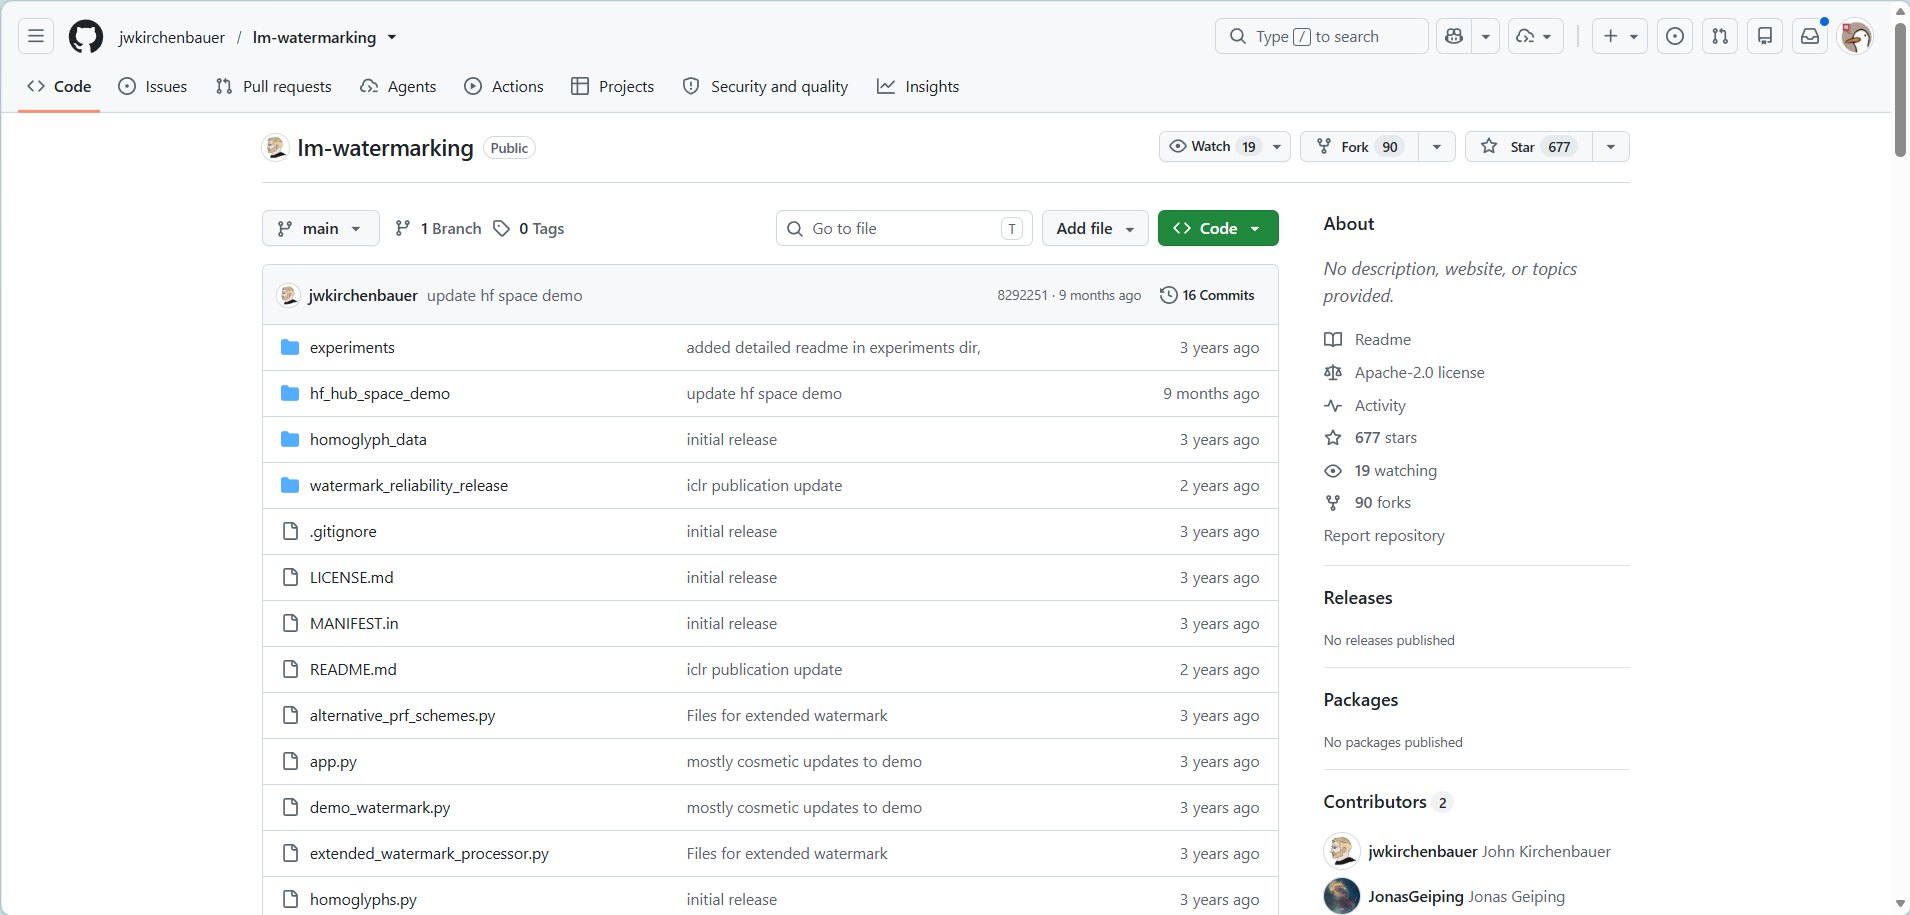
\includegraphics[width=0.92\textwidth]{official_repo.png}
    \caption{官方 lm-watermarking 仓库页面}
    \label{fig:official-repo}
\end{figure}

复现与后续实验基于 Anaconda 环境完成。正式实验环境使用 \texttt{pytorch} conda 环境，核心依赖包括 PyTorch、Transformers、datasets、scipy、pandas 和 matplotlib。模型方面，复现阶段先使用 \texttt{sshleifer/tiny-gpt2} 跑通官方 Demo，因为它下载快、显存压力小，适合排查环境和接口问题；确认生成、检测、CSV 输出和绘图流程没有问题后，先下载并使用 \texttt{facebook/opt-1.3b} 完成复现实验，再使用 \texttt{facebook/opt-2.7b} 进行后续改进方法比较。

\subsection{原始复现步骤}

官方复现按照“代码准备、依赖安装、模型下载、Demo 启动、结果验证”的顺序完成。复现阶段先用最小模型跑通完整链路，以便提前暴露 Gradio、Transformers 和模型加载接口的兼容性问题；随后使用本地模型启动官方 Gradio Demo，验证生成、检测和可视化链路。

复现过程中遇到的一个实际问题是 Gradio 版本兼容。官方旧代码中使用的 \texttt{demo.queue(concurrency\_count=3)} 在新版 Gradio 中已经不再兼容，启动时会报参数错误。将其改为 \texttt{demo.queue(default\_concurrency\_limit=3)} 后，前端页面可以正常打开。该修复本身不改变水印算法，只是让官方交互式 Demo 能在当前环境下运行。图~\ref{fig:official-demo-start} 展示了官方 Demo 正常启动后的界面。

\begin{figure}[H]
    \centering
    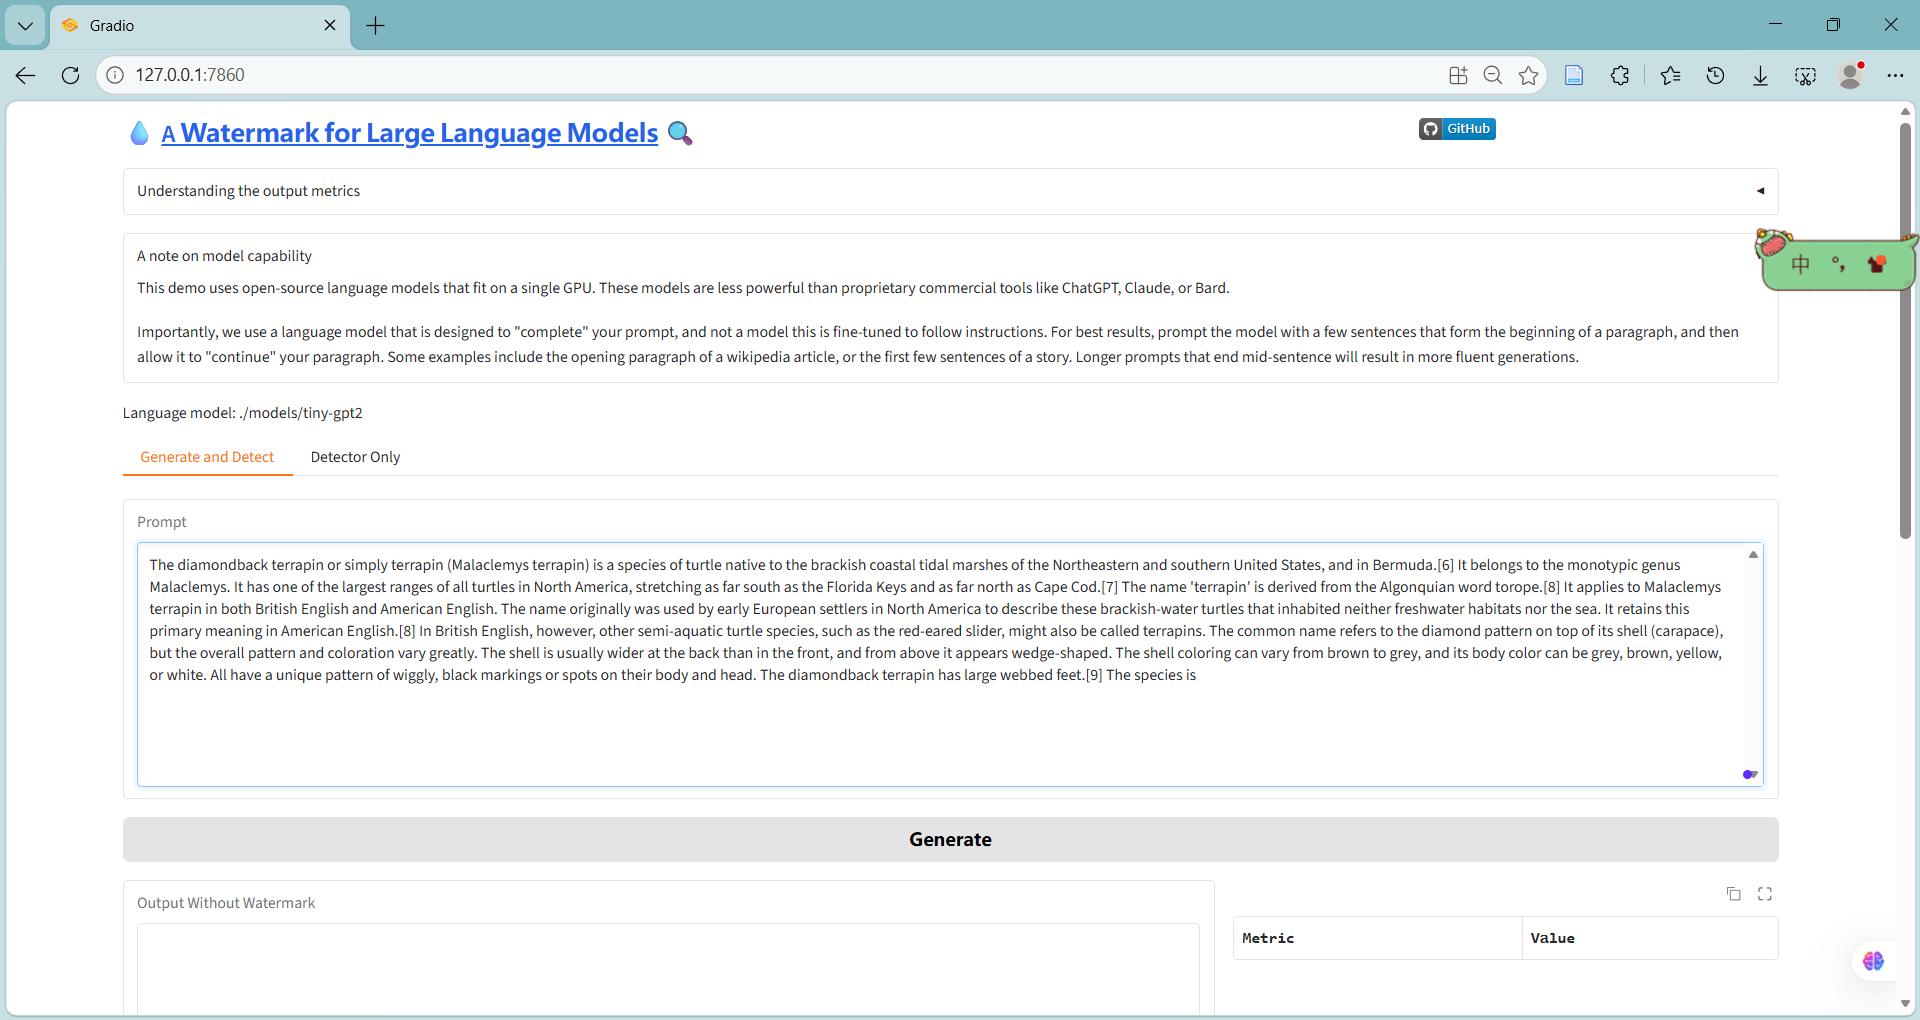
\includegraphics[width=0.92\textwidth]{official_demo_start.png}
    \caption{官方 Gradio Demo 启动界面}
    \label{fig:official-demo-start}
\end{figure}

\subsection{复现结果与验证}

官方 Demo 的验证方式很直接：输入同一个 prompt，系统同时生成无水印文本和带水印文本，并在右侧输出各自的检测统计量。一次典型复现结果如图~\ref{fig:official-demo-detection} 所示，无水印文本统计到 $T=99$ 个 token，其中 green token 数量为 22，\texttt{green\_fraction} 为 22.2\%，\texttt{z-score=-0.638}，检测结果为 \texttt{Human/Unwatermarked}；带水印文本统计到 $T=98$ 个 token，其中 green token 数量为 69，\texttt{green\_fraction} 为 70.4\%，\texttt{z-score=10.4}，检测结果为 \texttt{Watermarked}，置信度接近 100\%。

\begin{figure}[H]
    \centering
    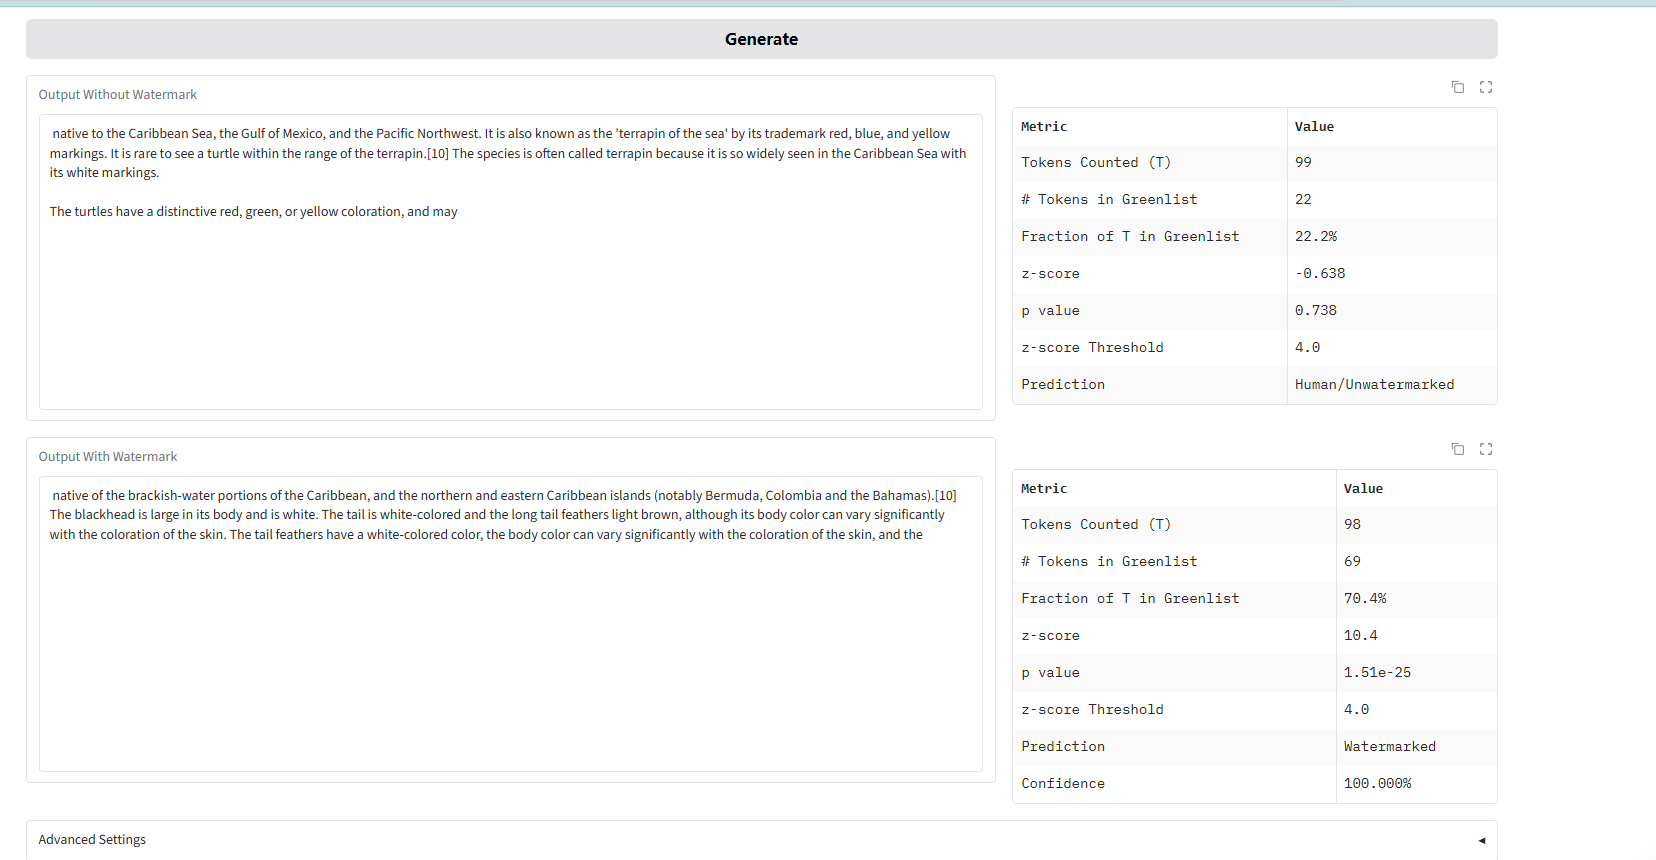
\includegraphics[width=0.92\textwidth]{official_demo_detection.png}
    \caption{官方 Demo 中无水印文本与带水印文本的检测结果}
    \label{fig:official-demo-detection}
\end{figure}

该结果展示了原论文方法的基本特征：水印并不是在文本表面添加某个特殊符号，而是在生成概率里持续施加很小的统计倾向；单个 token 看起来仍然自然，但几十个 token 累积后，green token 占比会显著偏离自然文本。也正因为这一点，z-score 成为后续实验最重要的检测指标之一。

\subsection{复现中观察到的问题}

完成官方 Demo 复现后，批量脚本进一步比较了不同固定 \texttt{delta} 的效果。\texttt{delta} 越大，green fraction 和 z-score 越高，检测成功率也越高；同时，强水印也会带来更明显的分布扰动。以 500 条 OPT-2.7B fp32 实验为例，\texttt{Fixed Delta 3.0} 的普通 KGW 检测成功率达到 98.40\%，平均 z-score 达到 10.0975，但 continuation PPL 升到 7.0199，明显高于无水印文本的 4.1244。\texttt{Fixed Delta 2.0} 的检测成功率为 92.80\%，PPL 为 5.4301；\texttt{Fixed Delta 1.7} 检测成功率为 82.00\%，PPL 为 4.9519。固定 \texttt{delta} 曲线提供了重要参照：强水印更容易检测，但流畅度和分布保持会付出代价。

固定 \texttt{delta} 的主要限制不在于检测能力不足，而在于它把所有生成位置当成一样处理。有些位置模型本来就非常确定，例如固定搭配、常见虚词或标点附近，强行推动 green token 更容易伤害自然性；有些位置模型有多个合理候选，此时嵌入水印的代价更低。原始方法没有区分这种差异，这构成了本文自适应水印方法的切入点。

\section{自适应水印方法设计}

\subsection{基于熵的 Adaptive Delta}

Adaptive Delta 方法利用 next-token 分布熵刻画当前位置的生成不确定性。对词表大小 $|V|$ 和原始 next-token 分布 $p_t$，实现中的归一化熵为
\[
    H_{\text{norm}}=-\frac{\sum_{v\in V}p_t(v)\log p_t(v)}{\log |V|}\in[0,1].
\]
当前实现固定 $\delta_{\min}=0.5$、$\delta_{\max}=3.0$、熵下界 $h_0=0.20$ 和指数 $\alpha=0.5$，并使用截断的凹映射
\[
    f(H_{\text{norm}})=\bigl(\max(H_{\text{norm}},h_0)\bigr)^\alpha.
\]
因此水印偏置为：
\[
    \delta_t=\delta_{\min}+(\delta_{\max}-\delta_{\min})\cdot f(H_{\text{norm}}).
\]
该映射先将熵截断到 $h_0$，再用 $\alpha<1$ 提升中等熵位置的偏置；最终值天然落在 $[\delta_{\min},\delta_{\max}]$ 内。它比固定 \texttt{delta} 更灵活，也具有直观解释：高熵位置有更多合理候选，适合使用更强水印；低熵位置更确定，适合使用较小偏置。

Adaptive Delta 的不足在于，熵到 \texttt{delta} 的映射仍然依赖经验参数，难以直接说明某个熵值对应某个具体偏置的分布意义。此外，若检测端仍然使用原始 KGW detector，则检测统计量没有显式利用生成端的可嵌入性差异。本文将 Adaptive Delta 作为重要对照方法，并进一步引入 KL 约束来重新定义每一步允许施加的水印强度。

\subsection{使用 KL 约束重新定义水印强度}

本文将水印强度控制改写为一个受约束的选择问题：每一步不直接指定 \texttt{delta}，而是在可接受的分布扰动预算内，选择尽可能大的水印偏置。设原始模型分布为 $P_t$，加水印后的分布为 $P'_t$，约束定义为：
\[
    D_{\mathrm{KL}}(P'_t\|P_t)\leq \varepsilon.
\]
该约束的含义是：水印可以改变模型分布，但这种改变不能超过预设预算 $\varepsilon$。在实现中，首先计算当前 greenlist 在原始分布下的概率质量 $p_G$，再对 $\delta_t$ 做二分搜索。对于给定 $\delta$，归一化因子为：
\[
    Z=1+(\exp(\delta)-1)p_G,
\]
加水印后 greenlist 的总概率质量为：
\[
    q_G=\frac{\exp(\delta)p_G}{Z},
\]
对应的 KL 散度可以写成：
\[
    D_{\mathrm{KL}}(P'_t\|P_t)=\delta q_G-\log Z.
\]
本文选择满足 KL 预算的最大 $\delta_t$。完整生成步骤为：先由当前 prefix 得到原始 logits 与 $P_t$；按 KGW 密钥构造 greenlist；计算 $p_G$；用 16 次二分搜索求满足预算的最大 $\delta_t$；将该偏置只加到 green token logits；最后按原采样参数采样 token。这样一来，水印强度不再由熵的经验映射给出，而是由当前分布和 KL 预算共同决定。小规模网格实验显示，$\varepsilon=0.02$ 时平均 \texttt{delta} 过低，检测信号不足；$\varepsilon=0.50$ 能使水印信号进入稳定可检出区间。在 500 条 OPT-2.7B fp32 实验中，\method{} 的平均自适应 \texttt{delta} 为 2.5108，既能形成明显水印痕迹，也保留了分布约束的解释。

\subsection{Candidate-aware Greenlist 与 Confidence Gate}

Candidate-aware Greenlist 不再直接在全词表中选 green token。实现先按 $P_t$ 从高到低排序，取累计概率首次达到 top-$p=0.95$ 的候选集合 $C_t$；再按与原 KGW 相同的 prefix seed 置乱整个词表，并保留其中属于 $C_t$ 的 token。greenlist 在候选集合内部按同一比例 $\gamma=0.25$ 取前 $\lfloor\gamma |C_t|\rfloor$ 个；若候选集合非空但该值为零，则退化为选取一个 token。候选集合外 token 不接收 logits 偏置，原 KGW 的密钥和置乱关系仍被保留。

Confidence Gate 的实际条件为
\[
    H_{\mathrm{norm}}\ge H_{\min}\quad\text{且}\quad p_{\mathrm{top1}}\le p_{\max}.
\]
正式 CA-KL-CG 采用 $(H_{\min},p_{\max})=(0.10,0.95)$。任一条件不满足时，该位置直接取 $\delta_t=0$，而不是使用较小偏置；满足条件时才执行上述 KL 二分搜索。这一设计将低熵或单一候选占主导的位置排除在嵌入之外。

\subsection{加权检测器的作用}

在生成端引入自适应强度后，检测端也需要相应调整。原始 z-score 把每个 token 位置等权看待，但在自适应水印中，每个位置的可嵌入性并不一样。为使检测器与生成机制更一致，本文实现了模型辅助的 entropy-weighted detector。检测时，系统用同一个基础模型重新计算每个 prefix 的 logits，得到当前位置的熵、候选 greenlist 及其概率质量，并对高熵位置赋予更高权重。

本文将生成端机制和检测端机制分开定义。\method{}、candidate-aware greenlist 和 confidence gate 属于生成端机制，决定文本如何被加水印；weighted detector 和 WinMax detector 属于检测端机制，决定同一段文本如何被评分。因此，``\method{} + Weighted Detector'' 表示对 \method{} 生成文本使用模型辅助检测器评分；完整方案可表述为 ``\fullmethod{} 生成 + weighted/WinMax 检测''。

加权检测的统计量为：
\[
    Z_w=\frac{\sum_i w_i(G_i-p_i)}
    {\sqrt{\sum_i w_i^2p_i(1-p_i)}}.
\]
其中 $G_i$ 表示第 $i$ 个生成 token 是否落入 greenlist，$p_i$ 是无水印条件下落入该 greenlist 的概率质量。实现取 $w_i=H_{\mathrm{norm},i}$；若该位置未通过 Confidence Gate，则令 $w_i=0$。权重未作额外归一化。由于 $w_i$ 只依赖当前 token 之前的 prefix，不依赖当前 token 是否命中 greenlist，这个统计量在无水印文本下仍然有合理的零均值解释。

此外，本文还实现了 windowed detector，即在每个连续窗口上计算局部加权 z-score，并取最大值：$Z_{\mathrm{WinMax}}=\max_{L\in\{20,40,80,\mathrm{max}\}}\max_s Z_w[s:s+L]$。这个设计主要面向 copy-paste 混入场景：如果一段带水印文本被插入到大量无水印文本中，全局统计量会被稀释，而窗口检测可以更容易发现局部水印片段。由于多窗口最大化会提高误报机会，WinMax 绝不能复用 weighted detector 的阈值；两种分数均须在独立 No Watermark 校准集上单独确定阈值。

\section{实现细节}

\subsection{项目结构与模块职责}

代码实现主要增加了三个部分。第一，生成与检测模块实现 CA-KL 生成器，负责 KL-constrained adaptive delta、confidence gate 和 candidate-aware greenlist。第二，该模块同时实现模型辅助检测器，负责 weighted z-score 和 WinMax weighted z-score。第三，批量实验模块统一执行 \texttt{No Watermark}、多个固定 \texttt{delta}、Adaptive Delta、\method{} 生成、\method{} + Candidate Greenlist 生成，以及 \fullmethod{} 生成，并分别记录普通 KGW 检测器和加权检测器的结果。

\begin{table}[H]
    \centering
    \caption{改进实验的功能模块与职责}
    \label{tab:code-structure}
    \small
    \begin{tabularx}{\textwidth}{p{0.48\textwidth}X}
        \toprule
        功能模块      & 作用                                       \\
        \midrule
        生成与检测模块   & CA-KL 生成、候选 greenlist、gate 与模型辅助检测       \\
        批量实验模块    & 统一生成、普通 KGW 检测，保存 prompt、文本与精确 token ids \\
        KL 预算扫描模块 & 500 条 KL 预算扫描、PPL 与校准                    \\
        局部混入攻击模块  & token 级局部混入攻击及三种检测器评分                    \\
        校准统计模块    & 五折阈值校准与 2000 次 bootstrap 置信区间            \\
        \bottomrule
    \end{tabularx}
\end{table}

\subsection{统一实验与结果记录}

实现中保持三个原则。首先，模型不做 fine-tuning，所有水印都在 inference-time 修改 logits，以保持方法与原论文设定一致。其次，保留普通 KGW 检测器，用于和固定 \texttt{delta} baseline 做同口径比较；模型辅助加权检测器则作为匹配 \method{} 和 \fullmethod{} 的增强检测口径。最后，结果分析脚本同时输出平均 z-score、普通检测成功率、AUC、TPR@1\%FPR、TPR@5\%FPR、平均 KL 和平均自适应 \texttt{delta} 等指标。每条新生成记录保存 \texttt{prompt\_id}、prompt、生成文本、精确 \texttt{token\_ids} 和检测分数；PPL 结果单独保存 continuation NLL 与 token 数，便于重新汇总而不覆盖原 CSV。

\subsection{可复现运行与断点续跑}

实验由统一的批处理入口执行，分别覆盖完整 baseline 对比、confidence gate 网格、选定 gate 下的 \method{} 系列、\texttt{Fixed Delta 1.7} 对照、KL 预算扫描与 copy-paste 攻击。每个任务均支持按已完成样本续跑，生成记录、PPL 记录、校准结果和图表输出分开保存。

为展示改进方法的实际运行效果，前端在同一 prompt 下同步生成无水印、Fixed Delta、\method{} 和 \fullmethod{} 文本，并即时计算标准 KGW、Weighted 和 WinMax 指标。图~\ref{fig:frontend-baseline} 展示输入 prompt 后的无水印与固定偏置输出；图~\ref{fig:frontend-cakl} 展示 \method{} 与 \fullmethod{} 的生成文本及逐条扰动统计；图~\ref{fig:frontend-summary} 汇总四种方法的即时检测结果。该前端用于呈现单条生成--检测流程，正式比较仍以第 6 节的 499 条 prompt 汇总与独立校准为准。

\begin{figure}[H]
    \centering
    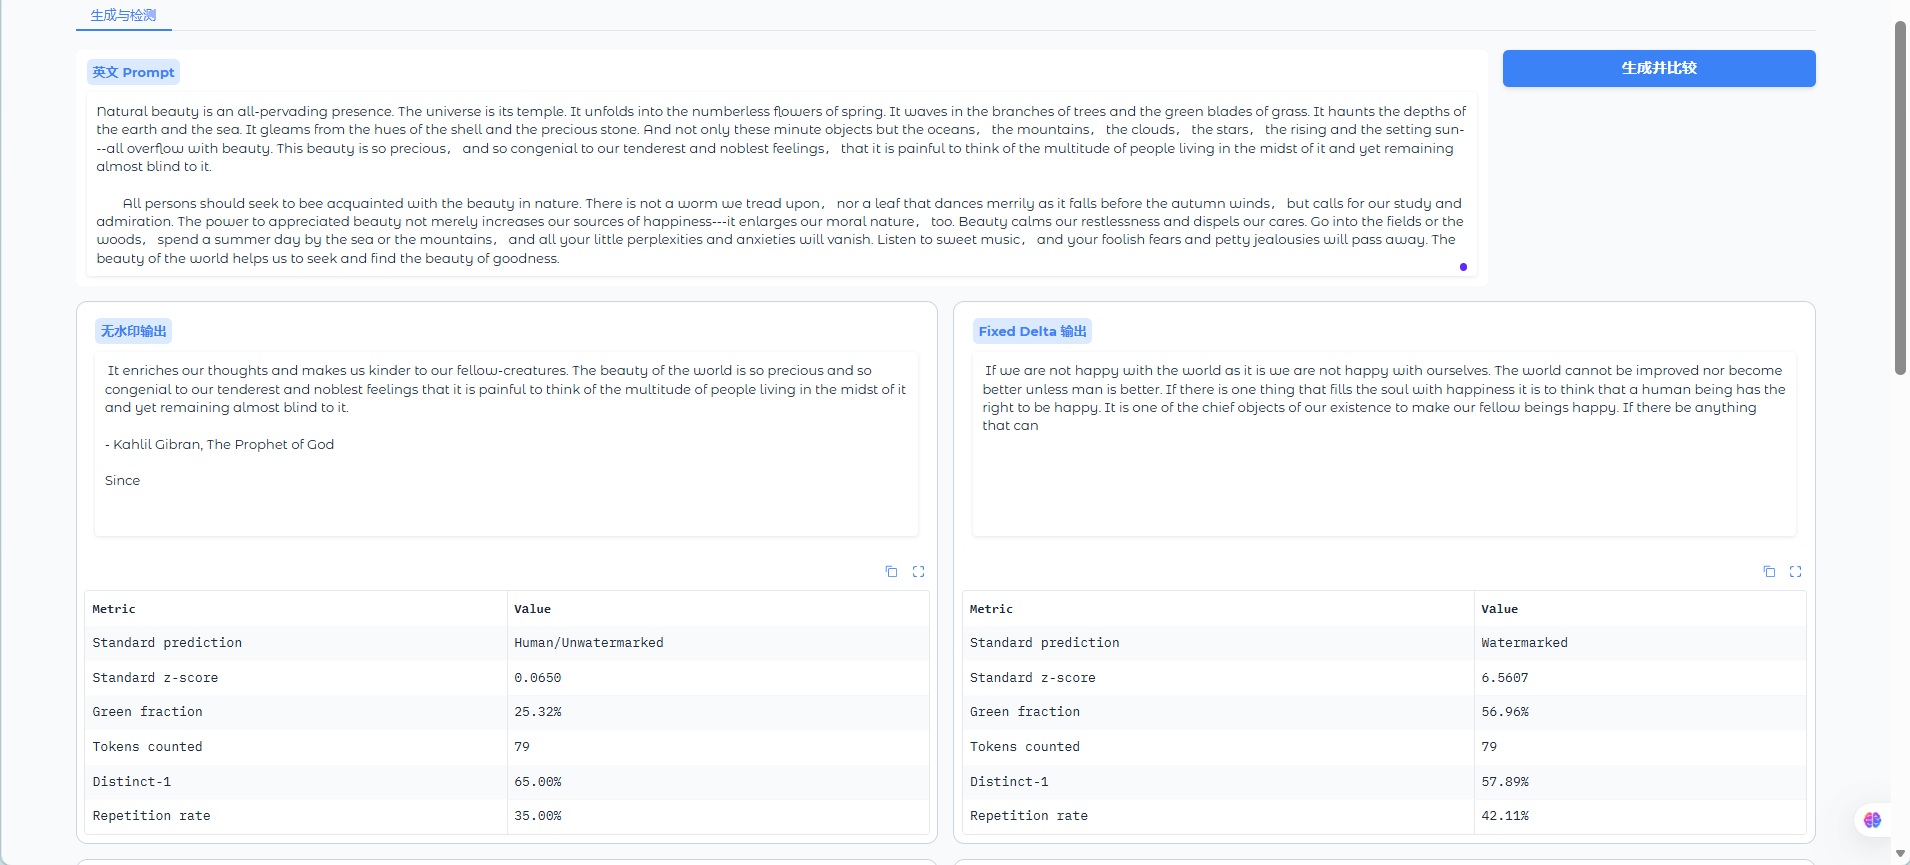
\includegraphics[width=0.96\textwidth]{frontend_baseline_comparison.png}
    \caption{前端中无水印与 Fixed Delta 的单条生成和标准 KGW 检测结果}
    \label{fig:frontend-baseline}
\end{figure}

\begin{figure}[H]
    \centering
    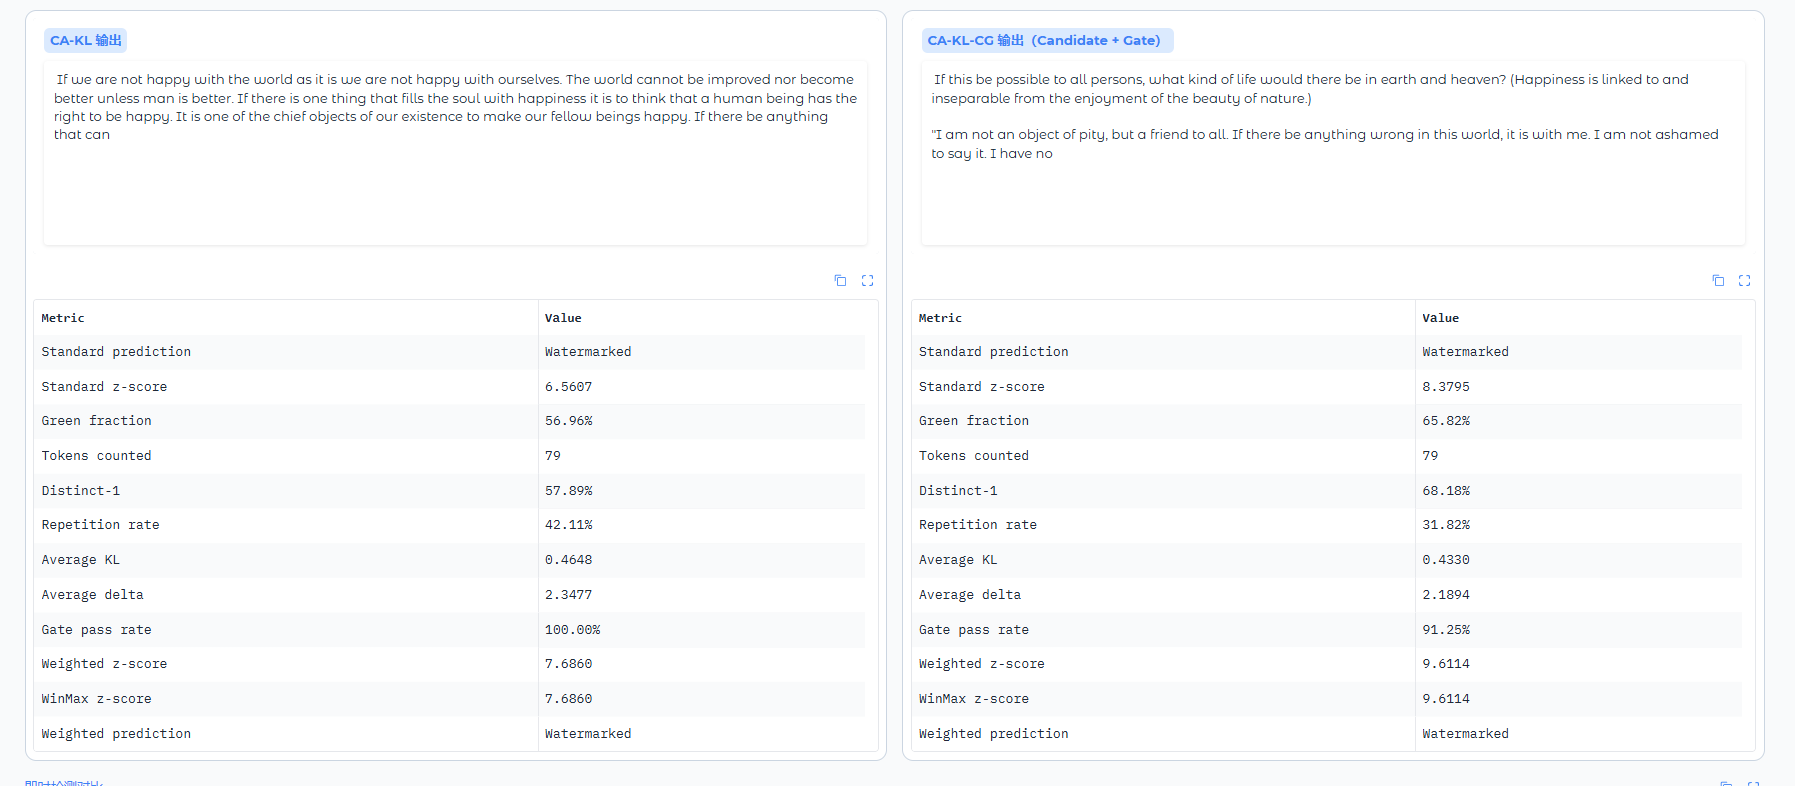
\includegraphics[width=0.96\textwidth]{frontend_cakl_comparison.png}
    \caption{前端中 CA-KL 与 CA-KL-CG 的生成、检测和扰动统计}
    \label{fig:frontend-cakl}
\end{figure}

\begin{figure}[H]
    \centering
    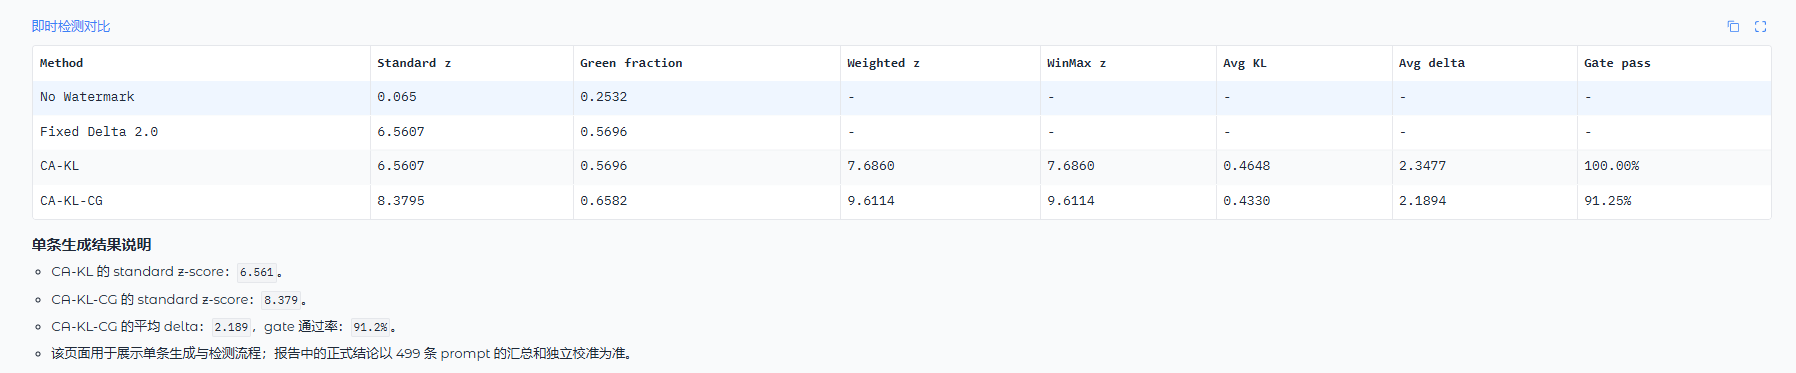
\includegraphics[width=0.96\textwidth]{frontend_detection_summary.png}
    \caption{前端对四种生成策略的即时检测汇总}
    \label{fig:frontend-summary}
\end{figure}

\section{实验设置}

\subsection{原论文复现实验}

本报告把实验拆成两层。第一层是严格对齐原论文口径的 KGW 复现实验：使用 \texttt{facebook/opt-1.3b}、C4/realnewslike、500 条固定随机种子打乱后抽取的 prompt、论文风格的 prompt 构造，以及 200$\pm$5 个有效 scored tokens 的生成长度控制，并仅采用 standard KGW detector。第二层才是本文改进方法实验：使用 \texttt{facebook/opt-2.7b}、500 条样本、普通 KGW detector 与匹配 weighted detector，系统比较 Adaptive Delta、\method{} 和 \fullmethod{}。

\begin{table}[H]
    \centering
    \caption{复现实验设置}
    \label{tab:setup}
    \begin{tabularx}{0.92\textwidth}{p{0.30\textwidth}X}
        \toprule
        项目        & 设置                                                                       \\
        \midrule
        基础模型      & \texttt{facebook/opt-1.3b}                                               \\
        数据集       & \texttt{C4/realnewslike}                                                 \\
        正式评估样本数   & 500 条 prompt                                                             \\
        Prompt 构造 & shuffle + fixed seed=1234；从样本文本末尾裁掉固定 200-token completion，剩余前缀作为 prompt \\
        生成长度控制    & target new tokens = 200，要求 \texttt{tokens\_scored} 接近 200$\pm$5          \\
        采样方式      & multinomial sampling，temperature = 0.7                                   \\
        水印比例参数    & $\gamma=0.25$                                                            \\
        正式水印线     & \texttt{Fixed Delta 2.0}                                                 \\
        检测口径      & standard KGW detector，z-score threshold = 4.0                            \\
        PPL 评分    & 使用无水印 \texttt{OPT-2.7B} 仅对 continuation 评分                               \\
        硬件        & 共享服务器单卡 GPU                                                              \\
        \bottomrule
    \end{tabularx}
\end{table}

\subsection{受控改进方法比较}

为检验改进而非模型规模或 prompt 差异的影响，受控改进实验固定 OPT-1.3B、上述 500 条 paper-style prompt、200$\pm$5 tokens、temperature 0.7、$\gamma=0.25$、FP32 与 standard KGW detector，只改变水印强度控制机制。PPL 统一由无水印 OPT-2.7B 对 continuation 评分，以避免评价器随生成方法改变。比较对象包括 No Watermark、Fixed Delta 2.0、Adaptive Delta、\method{}、Candidate Greenlist 和 \fullmethod{}。

\subsection{Pareto 与消融实验}

扩展实验在 OPT-2.7B 上扫描 $\varepsilon\in\{0.20,0.30,0.35,0.40,0.50\}$，并保留 Fixed Delta 曲线，以分析 KL 预算的质量--检测控制关系。Candidate Greenlist 与 confidence gate 的作用通过相同 prompt 上的消融、gate 网格和逐位置 \texttt{delta} 统计进行分析；这些结果作为机制分析，而非替代第 5.2 节的受控主比较。

\subsection{鲁棒性与校准实验}

鲁棒性实验将已有生成结果在 token 级拼接为 200-token copy-paste 攻击，覆盖 0/25/50/75/100\% 水印比例与 beginning/middle/end 插入位置。独立校准实验按 \texttt{prompt\_id} 五折划分：每折以 400 条 No Watermark 样本确定阈值，在剩余 100 条负样本和同索引水印文本上评估，并采用 2000 次 bootstrap 给出 95\% 置信区间。

\subsection{评价指标}

评价指标分为三类。第一类是原始 KGW 检测指标，包括 green fraction、普通 z-score 和普通 detection success rate；其中 success rate 指文本在原始 KGW 检测器下被判定为 \texttt{Watermarked} 的比例。第二类是文本质量指标，包括 continuation PPL、Distinct-1、Distinct-2 和 Repetition Rate；PPL 越低说明生成文本越接近原模型分布，Distinct 越高通常说明文本越不重复，Repetition Rate 越低说明词汇重复越少。第三类是匹配自适应生成机制的增强检测指标，包括 Weighted z-score、WinMax Weighted z-score、AUC 和 TPR@FPR。这三类指标回答的问题不同：普通 KGW 指标衡量与原论文检测器的兼容性，加权检测指标衡量模型辅助检测是否能捕捉自适应水印信号，质量指标衡量生成扰动带来的副作用。

\section{实验结果}

\subsection{复现实验主表}

\begin{table}[H]
    \centering
    \caption{OPT-1.3B + C4/realnewslike + 200$\pm$5 tokens + standard KGW detector 的复现结果}
    \label{tab:main-results}
    \scriptsize
    \setlength{\tabcolsep}{2.5pt}
    \begin{tabularx}{\textwidth}{p{0.24\textwidth}rrrrrrr}
        \toprule
        生成方法            & KGW z            & KGW 检出率          & Green Frac.     & Avg Tokens      & Corpus PPL      & Distinct-1      & 重复率             \\
        \midrule
        No Watermark    & -0.2836          & 0.20\%           & 0.2414          & 203.82          & \textbf{3.8492} & \textbf{0.5571} & \textbf{0.4429} \\
        Fixed Delta 2.0 & \textbf{10.6006} & \textbf{96.19\%} & \textbf{0.5714} & \textbf{203.96} & 4.9195          & 0.5374          & 0.4626          \\
        \bottomrule
    \end{tabularx}
\end{table}

表 \ref{tab:main-results} 被前置为本报告主表，是因为它和原论文口径最接近：模型固定为 \texttt{OPT-1.3B}，数据集固定为 C4/realnewslike，检测器固定为 standard KGW detector，生成长度也稳定控制在 200 token 量级。结果显示，\texttt{Fixed Delta 2.0} 能把平均 z-score 从 $-0.2836$ 提高到 $10.6006$，把检出率从 0.20\% 提高到 96.19\%，同时 green fraction 从 0.2414 提高到 0.5714，说明我们已经复现出与原论文一致的核心统计趋势。
从质量指标看，\texttt{Fixed Delta 2.0} 的 continuation PPL 从 3.8492 上升到 4.9195，Distinct-1 从 0.5571 下降到 0.5374，重复率从 0.4429 上升到 0.4626。这说明原论文的基本现象也被同步复现出来了：固定偏置确实容易检测，但会带来可观测的分布扰动和一定的文本质量损失。

\begin{figure}[H]
    \centering
    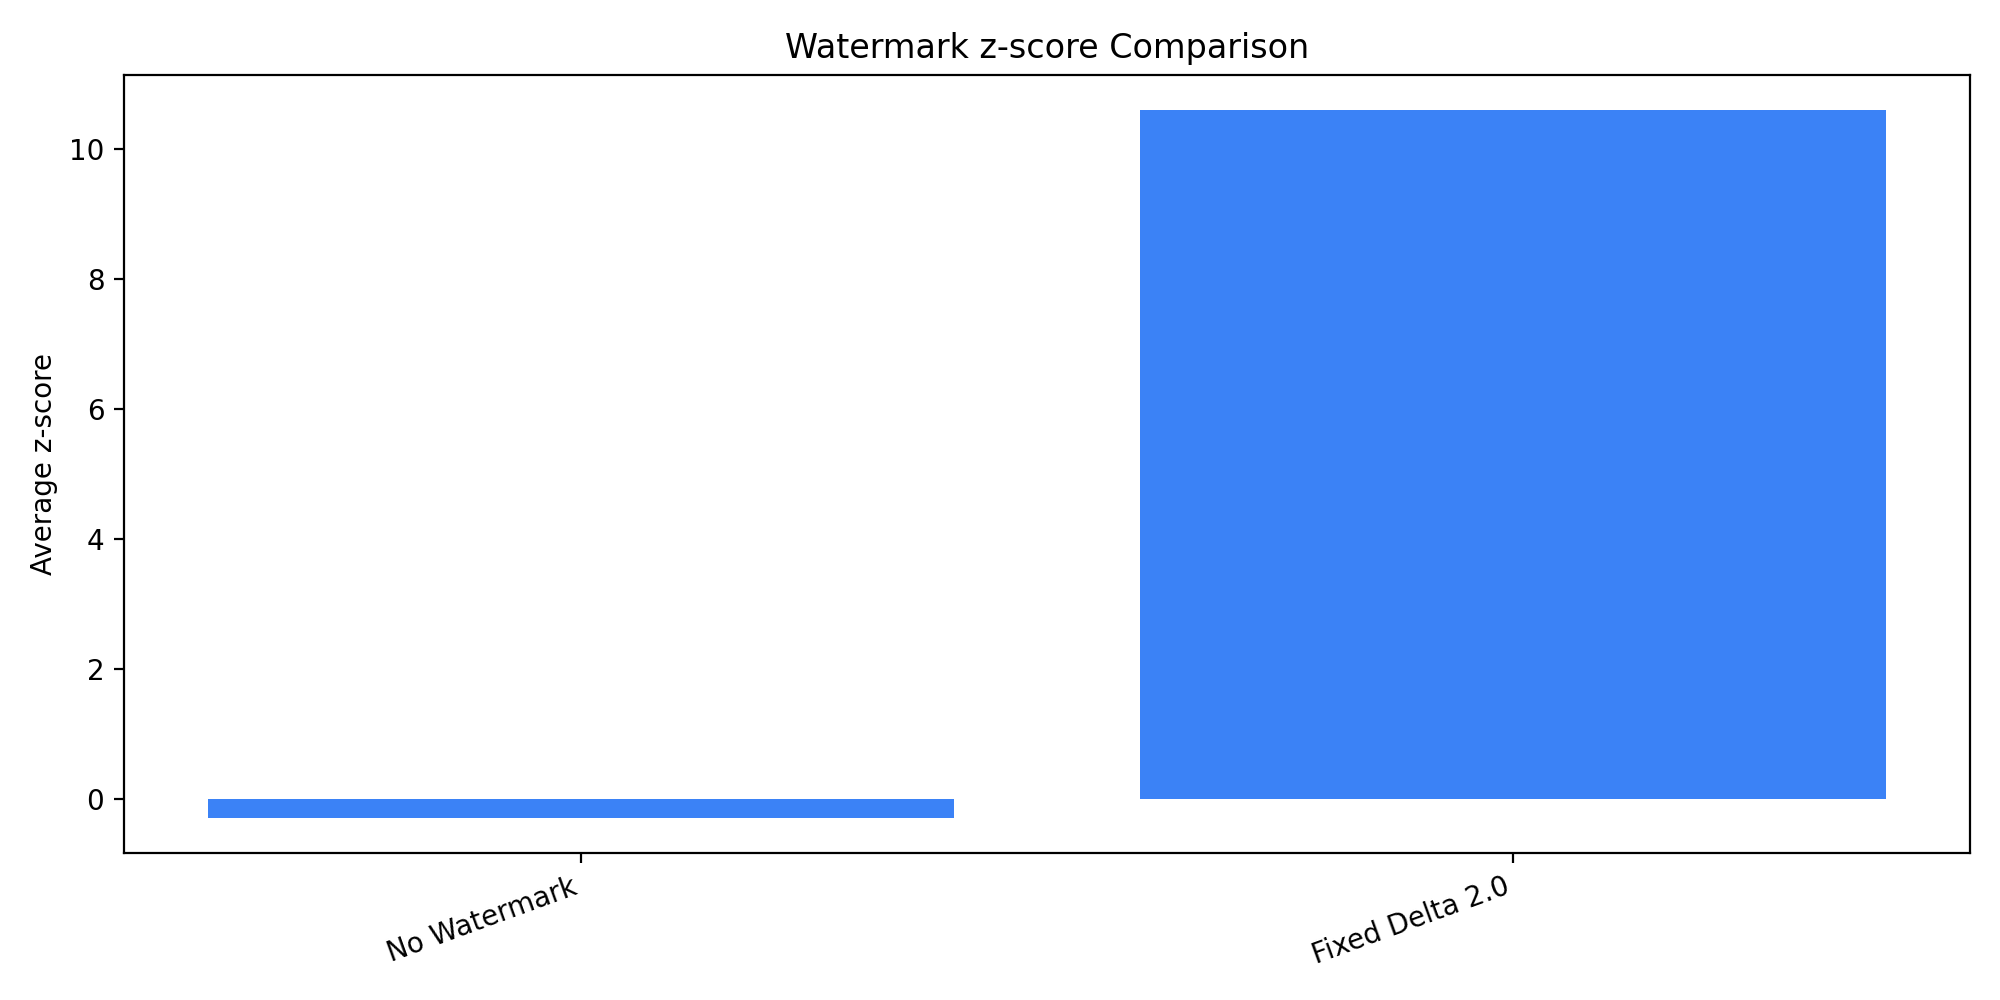
\includegraphics[width=0.86\textwidth]{opt13b_paper_zscore.png}
    \caption{复现实验中 standard KGW detector 的平均 z-score 对比}
    \label{fig:paper-zscore}
\end{figure}

\begin{figure}[H]
    \centering
    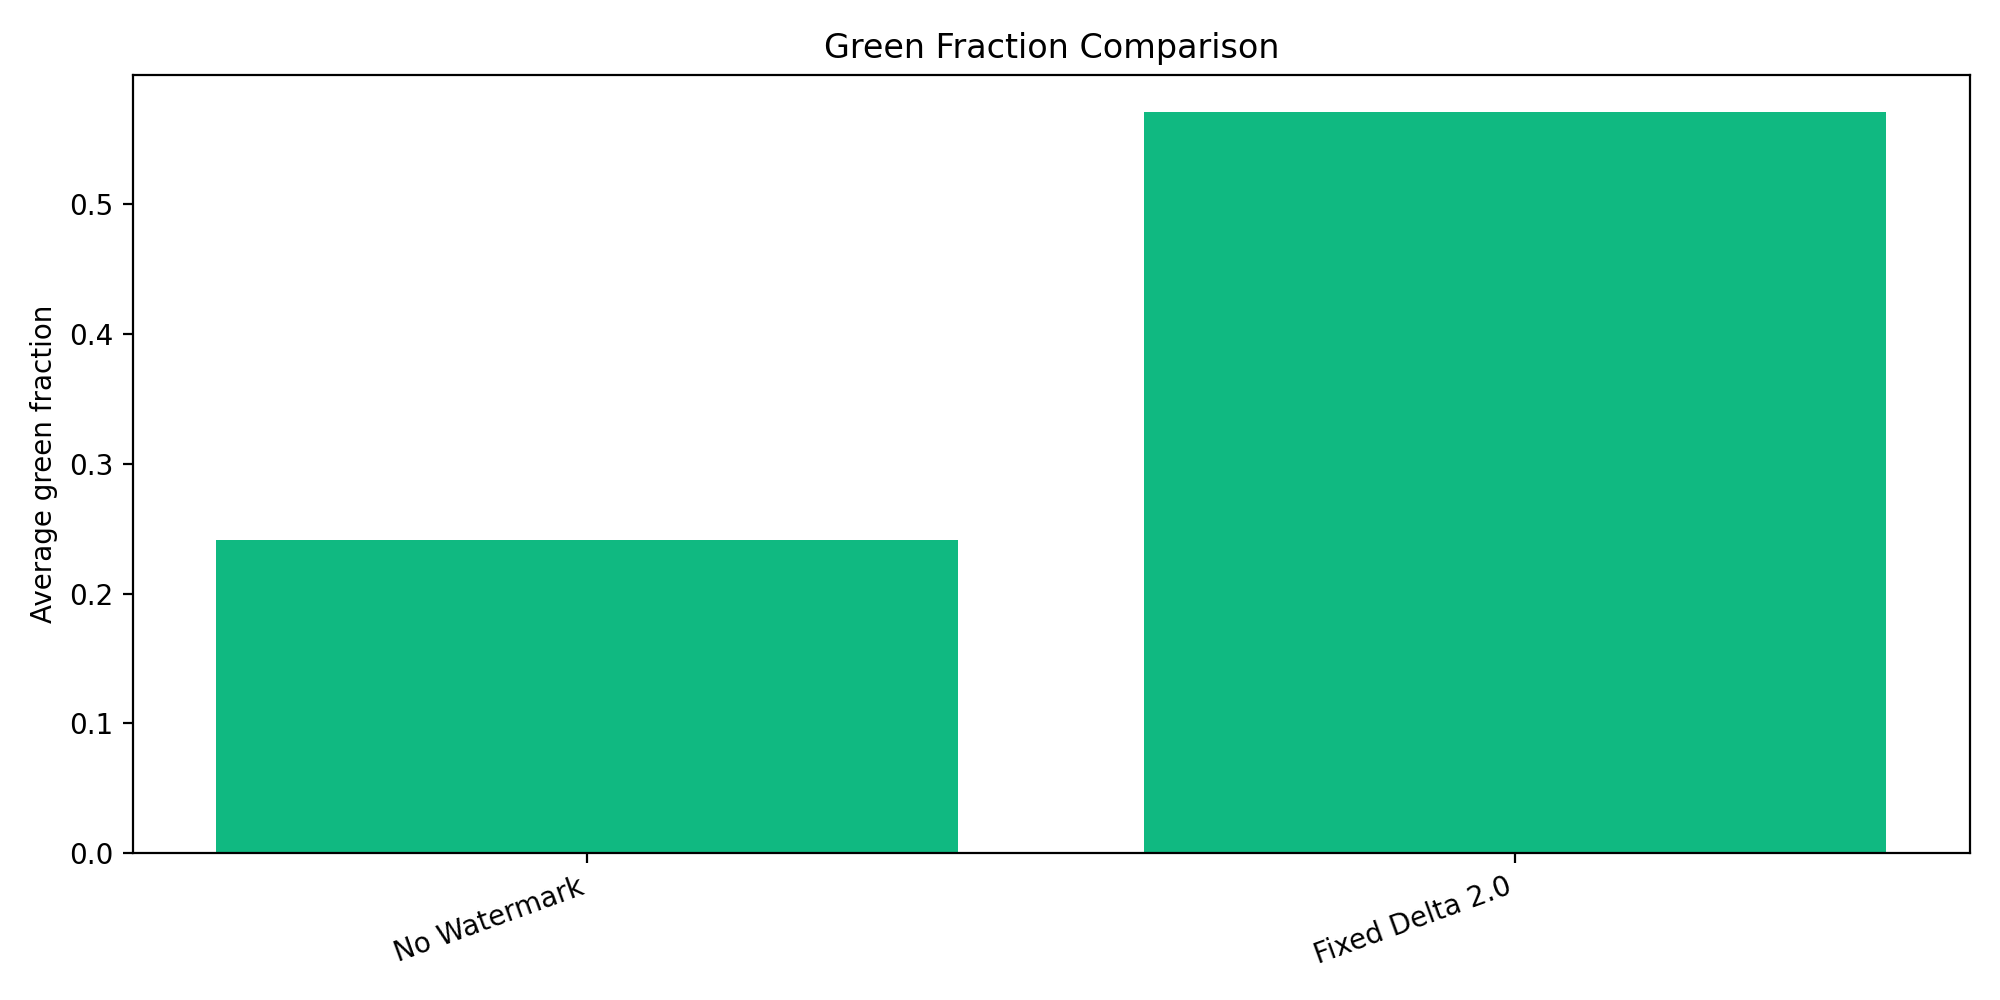
\includegraphics[width=0.86\textwidth]{opt13b_paper_green.png}
    \caption{复现实验中 standard KGW detector 的 green fraction 对比}
    \label{fig:paper-green}
\end{figure}

\subsection{原论文控制变量下的改进方法}

\begin{table}[H]
    \centering
    \caption{控制变量下的改进方法比较：OPT-1.3B、499 个有效 C4/realnewslike prompt、200$\pm$5 token；PPL 统一由 OPT-2.7B 评测}
    \label{tab:improved-results}
    \scriptsize
    \setlength{\tabcolsep}{2.5pt}
    \begin{tabularx}{\textwidth}{p{0.31\textwidth}rrrrrr}
        \toprule
        生成方法                         & KGW z            & KGW 检出率          & Corpus PPL      & 平均 KL  & 平均 $\delta$ & 重复率             \\
        \midrule
        No Watermark                 & -0.1264          & 1.00\%           & \textbf{4.5207} & --     & --          & \textbf{0.4413} \\
        Fixed Delta 2.0              & 10.6572          & 97.39\%          & 5.7426          & --     & 2.0000      & 0.4709          \\
        Adaptive Delta               & 9.9697           & 96.79\%          & 5.5995          & --     & --          & 0.4685          \\
        \method{}                    & \textbf{12.1205} & \textbf{98.40\%} & 6.3104          & 0.3642 & 2.5401      & 0.4728          \\
        \fullmethod{}，gate 0.10/0.95 & 10.4528          & 97.19\%          & 6.1984          & 0.3327 & 1.6304      & 0.4614          \\
        \bottomrule
    \end{tabularx}
\end{table}

表 \ref{tab:improved-results} 在统一实验条件下报告五类具有代表性的生成策略：无水印文本用于估计标准 KGW 检测器的背景分数；Fixed Delta 2.0 对齐原始 KGW 的固定偏置设定；Adaptive Delta 检验基于熵的动态强度控制；\method{} 检验逐位置 KL 预算约束；\fullmethod{} 则同时考察 candidate-aware greenlist 与 confidence gate 对 KL 约束生成的影响。所有生成与普通检测均在相同的 499 个 prompt 上完成，PPL 则由独立的未加水印 OPT-2.7B 统一重算，因而方法间可直接比较。

\method{} 的普通 KGW z-score 和检出率最高，分别为 12.1205 和 98.40\%，但其 PPL 为 6.3104，高于 Fixed Delta 的 5.7426。加入 confidence gate 后，\fullmethod{} 的平均 \texttt{delta} 从 2.5401 降至 1.6304，实际施加水印的位置占 69.44\%，PPL 下降到 6.1984，而普通检出率仍为 97.19\%。这支持其作为“降低嵌入覆盖率的折中方案”，而非优于全部基线的严格 Pareto 支配方案。

按 \texttt{prompt\_id} 进行五折独立阈值校准时，\method{} 的 standard z-score AUC 为 0.9954，TPR@1\%FPR 为 98.40\%（实际 FPR 1.40\%）；\fullmethod{} 的对应值为 0.9926 和 97.19\%。因此，上述检测结论并非复用同一批负样本的阈值与评估，而是由每折未参与阈值确定的 No Watermark 样本评测得到。

\subsection{扰动控制与门控参数消融}

Confidence gate 控制 \fullmethod{} 的实际嵌入位置：只有当当前位置满足熵下界且 top-1 概率不超过给定阈值时，生成器才施加水印偏置。为了分析 gate 对水印强度的影响，实验比较了五组 $(H_{\text{norm}},p_{\text{top1}})$ 参数。结果见表 \ref{tab:gate-grid}。

\begin{table}[H]
    \centering
    \caption{50 条样本上 \fullmethod{} 的 confidence gate 网格结果}
    \label{tab:gate-grid}
    \scriptsize
    \setlength{\tabcolsep}{3pt}
    \begin{tabularx}{\textwidth}{p{0.18\textwidth}rrrrrr}
        \toprule
        Gate $(H,p_{\text{top1}})$ & KGW 检出率       & Weighted 检出率  & KGW z           & Weighted z      & 平均 $\delta$     & Gate 通过率        \\
        \midrule
        0.10 / 0.95                & \textbf{78\%} & 96\%          & \textbf{5.8227} & \textbf{8.6790} & \textbf{1.6579} & \textbf{0.7066} \\
        0.20 / 0.95                & 72\%          & 96\%          & 5.1175          & 8.3224          & 1.1745          & 0.5214          \\
        0.25 / 0.90                & 58\%          & \textbf{98\%} & 4.1687          & 7.5757          & 0.9182          & 0.4123          \\
        0.30 / 0.90                & 26\%          & 96\%          & 2.9042          & 6.7417          & 0.6477          & 0.2967          \\
        0.35 / 0.85                & 20\%          & 84\%          & 2.3187          & 5.8281          & 0.4585          & 0.2120          \\
        \bottomrule
    \end{tabularx}
\end{table}

表 \ref{tab:gate-grid} 表明，gate 越严格，平均 \texttt{delta}、gate 通过率和普通 KGW z-score 越低。0.10/0.95 在网格实验中取得最高的普通 KGW 检出率，并保持 96\% 的 weighted 检出率，因此作为 \fullmethod{} 的正式实验参数。

\subsection{匹配检测与独立阈值校准}

由于 \method{} 和 \fullmethod{} 的生成强度是动态变化的，原始 z-score 只能反映一部分信息。普通 KGW 检测器默认所有位置等权，但 \fullmethod{} 会通过 candidate-aware greenlist 和 confidence gate 选择更适合嵌入的位置，因此检测端也应当利用这些位置差异。表 \ref{tab:weighted} 比较了 weighted z-score 和 WinMax weighted z-score 的结果。

\begin{table}[H]
    \centering
    \caption{不同生成文本在模型辅助加权检测器下的诊断指标}
    \label{tab:weighted}
    \scriptsize
    \setlength{\tabcolsep}{3pt}
    \begin{tabularx}{\textwidth}{p{0.32\textwidth}rrrrrr}
        \toprule
        生成文本 / 检测口径                     & Weighted z      & WinMax z        & Weighted 检出率     & 平均 KL           & 平均 $\delta$     & Gate 通过率 \\
        \midrule
        No Watermark                    & 0.1427          & 1.7069          & 0.00\%           & --              & --              & 0.7084   \\
        \method{} + Weighted Detector   & 8.8399          & 8.8749          & \textbf{97.60\%} & 0.3828          & 2.5108          & 1.0000   \\
        CA-KL + Candidate Greenlist     & \textbf{9.1410} & \textbf{9.1789} & 96.60\%          & 0.3904          & 2.4861          & 0.7302   \\
        \fullmethod{} + Weighted/WinMax & 9.1174          & 9.1552          & \textbf{97.60\%} & \textbf{0.3481} & \textbf{1.6893} & 0.7230   \\
        \bottomrule
    \end{tabularx}
\end{table}

表 \ref{tab:weighted} 中的 weighted detector 只改变检测统计量，不改变生成文本。\method{} 与 \method{} + Weighted Detector 使用同一批生成结果，\fullmethod{} 也是先完成生成，再用 weighted/WinMax detector 评分。因此，该检测器的作用主要体现在 weighted z-score、AUC 和 TPR@FPR 上。\fullmethod{} 的平均 \texttt{delta} 为 1.6893，低于 \method{} 的 2.5108，但 weighted 检出率达到 97.60\%，weighted z-score 达到 9.1174。这说明 \fullmethod{} 能将水印信号集中到更适合嵌入和检测的位置，使模型辅助检测器获得更强的统计证据。

\begin{table}[H]
    \centering
    \caption{同批 No Watermark 负样本上的初步加权检测质量（仅作诊断）}
    \label{tab:auc}
    \scriptsize
    \setlength{\tabcolsep}{2.5pt}
    \begin{tabularx}{\textwidth}{p{0.18\textwidth}p{0.30\textwidth}rrr}
        \toprule
        检测分数       & 生成文本 / 检测口径                     & AUC             & TPR@1\%FPR       & TPR@5\%FPR       \\
        \midrule
        Weighted z & CA-KL + Candidate Greenlist     & 0.9988          & 99.00\%          & 99.20\%          \\
        Weighted z & \method{} + Weighted Detector   & \textbf{0.9994} & 99.40\%          & \textbf{99.60\%} \\
        Weighted z & \fullmethod{} + Weighted/WinMax & 0.9992          & \textbf{99.60\%} & \textbf{99.60\%} \\
        WinMax z   & CA-KL + Candidate Greenlist     & 0.9938          & 97.60\%          & 98.40\%          \\
        WinMax z   & \method{} + Weighted Detector   & 0.9952          & 98.00\%          & 98.20\%          \\
        WinMax z   & \fullmethod{} + Weighted/WinMax & \textbf{0.9970} & \textbf{98.20\%} & \textbf{99.20\%} \\
        \bottomrule
    \end{tabularx}
\end{table}

表 \ref{tab:auc} 使用同一批 No Watermark 分数确定阈值并计算 TPR，因此只保留为便于与旧实验对照的诊断结果，不能作为低误报率泛化性能的正式结论。下面采用按 \texttt{prompt\_id} 划分的独立五折校准结果替代该口径。

对 500 条固定 prompt，本文以种子 1234 划分 5 折；每折仅用 400 条 No Watermark 分数分别为 KGW、weighted 和 WinMax 分数确定 99/95 分位阈值，再在剩余 100 条负样本上测量实际 FPR，并在相同 prompt id 的水印文本上计算 TPR。所有区间采用 2000 次 bootstrap 的 95\% 置信区间。表 \ref{tab:calibrated-final} 给出完整方案的 out-of-fold 结果；每折样本数为 100，因此实际 FPR 会围绕目标值以 1\% 的离散粒度波动。

\begin{table}[H]
    \centering
    \caption{\fullmethod{} 的五折独立校准结果（500 条，95\% CI）}
    \label{tab:calibrated-final}
    \scriptsize
    \setlength{\tabcolsep}{3pt}
    \begin{tabularx}{\textwidth}{p{0.14\textwidth}p{0.20\textwidth}p{0.20\textwidth}rp{0.20\textwidth}r}
        \toprule
        分数         & AUC（95\% CI）            & TPR@1\%FPR（95\% CI）      & 实际 FPR & TPR@5\%FPR（95\% CI）      & 实际 FPR \\
        \midrule
        Weighted z & 0.9992 [0.9977, 1.0000] & 99.60\% [99.0\%, 100\%]  & 1.40\% & 99.60\% [99.0\%, 100\%]  & 5.20\% \\
        WinMax z   & 0.9970 [0.9931, 0.9996] & 98.20\% [96.8\%, 99.2\%] & 1.00\% & 99.20\% [98.4\%, 99.8\%] & 5.20\% \\
        \bottomrule
    \end{tabularx}
\end{table}

\fullmethod{} 的 continuation PPL bootstrap 估计为 5.6037，95\% CI 为 [5.3892, 5.8100]；对应 No Watermark 为 4.1253 [4.0054, 4.2552]。因此，现有结果支持“匹配检测器对该生成文本具有较强区分能力”，但不应将同批校准的初步表述为严格的目标 FPR；后续 Pareto 与 copy-paste 实验沿用相同的交叉校准脚本。

\begin{figure}[H]
    \centering
    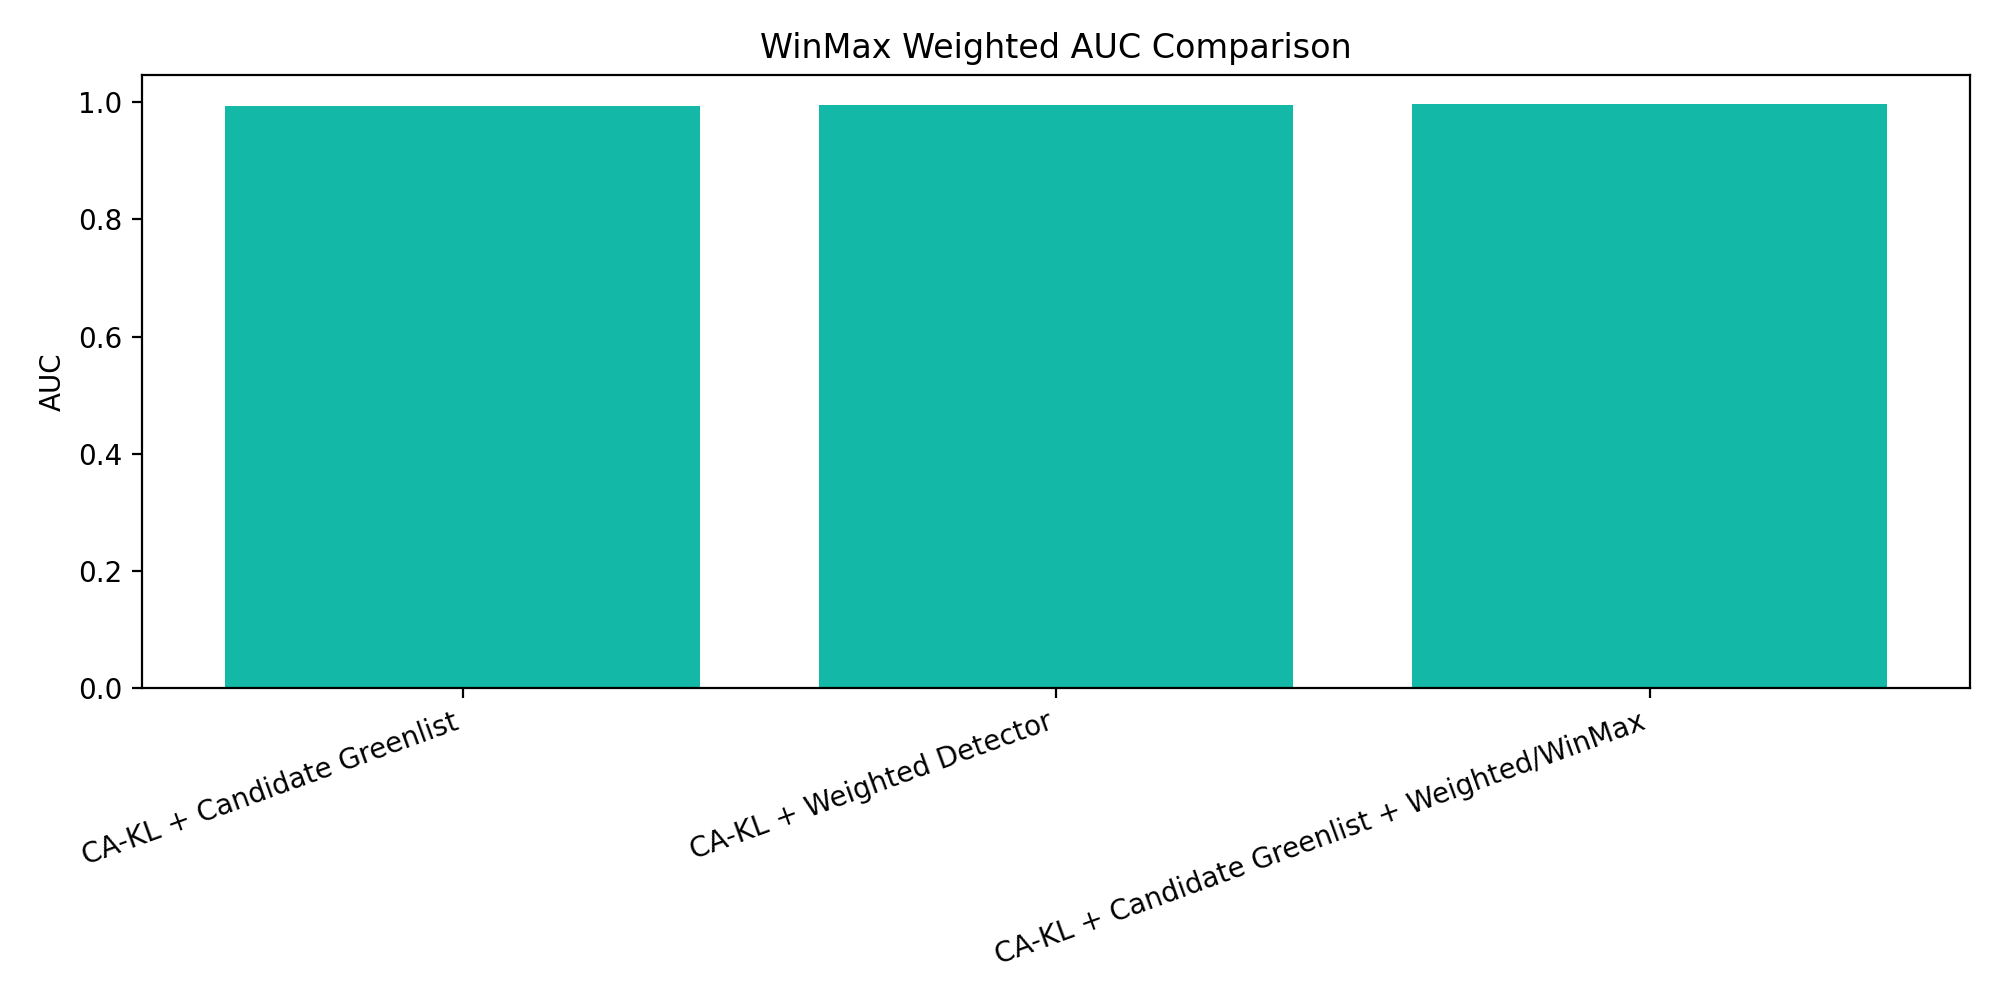
\includegraphics[width=0.86\textwidth]{cakl_weighted_auc.png}
    \caption{选定 gate 0.10/0.95 下 CA-KL 系列的 weighted AUC 对比}
    \label{fig:weighted-auc}
\end{figure}

\begin{figure}[H]
    \centering
    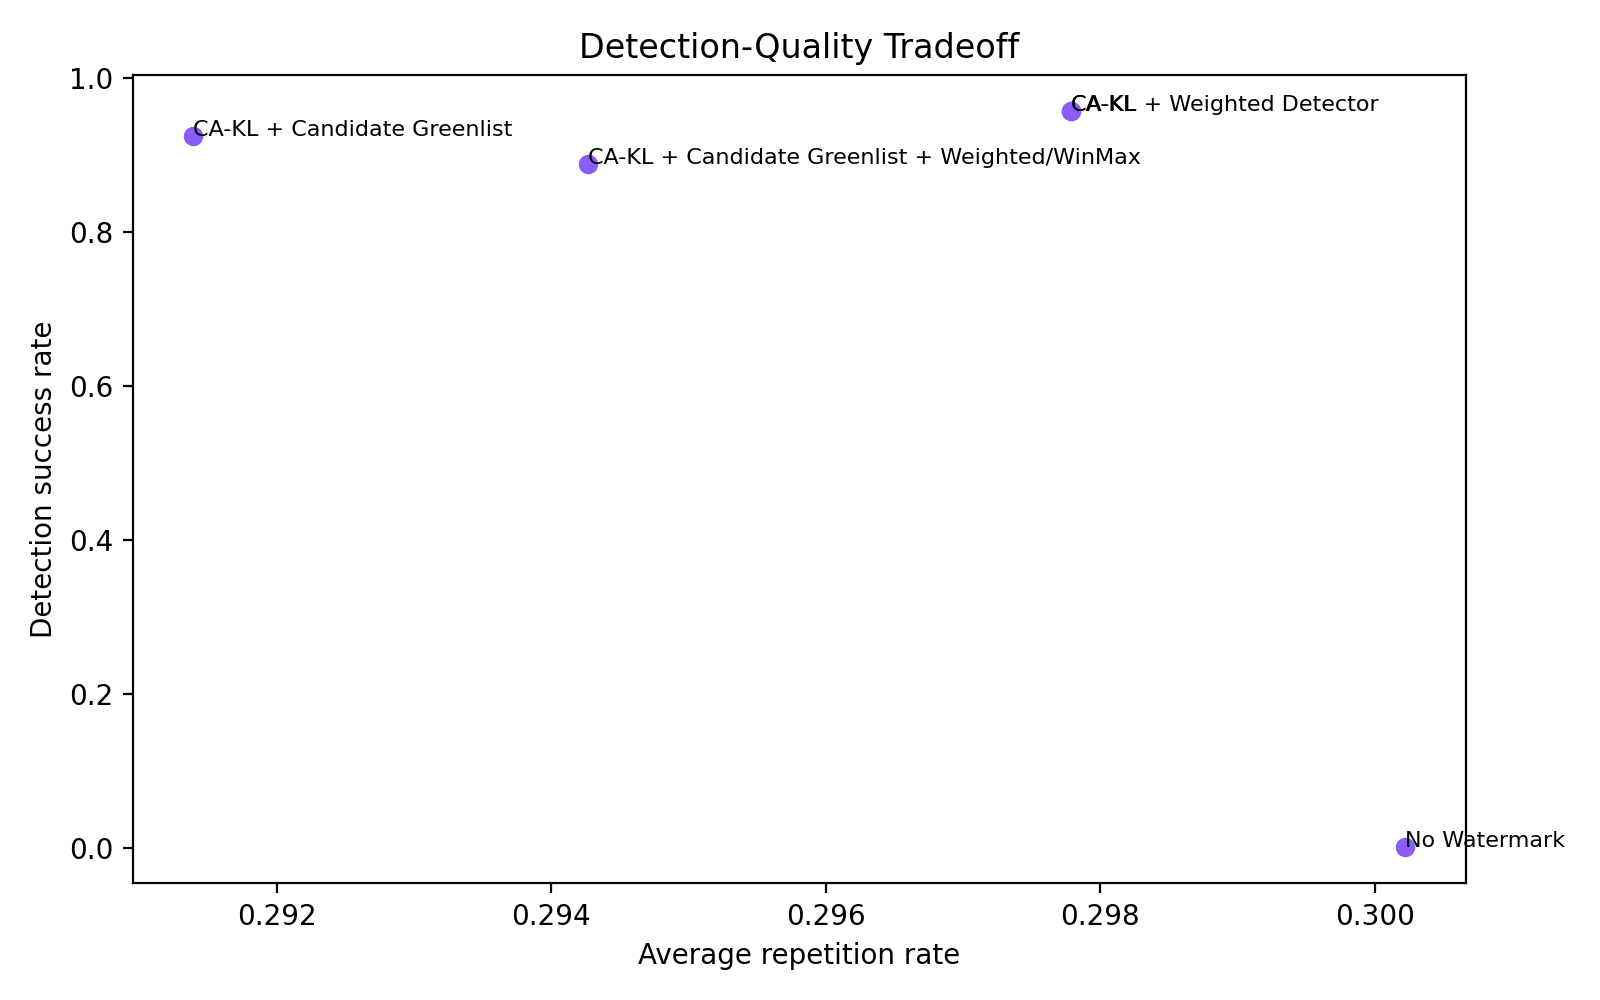
\includegraphics[width=0.86\textwidth]{cakl_tradeoff.png}
    \caption{选定 gate 0.10/0.95 下 CA-KL 系列的检测率与重复率折中}
    \label{fig:tradeoff}
\end{figure}

\subsection{KL 预算扫描、Pareto 与局部混入鲁棒性}

KL 预算 $\varepsilon$ 直接控制每一步允许的分布扰动。小规模网格实验比较了 $\varepsilon=0.30,0.35,0.40,0.50$；当 $\varepsilon$ 过小时，平均 \texttt{delta} 较低，水印信号不足。$\varepsilon=0.50$ 能使 \method{} 的平均 \texttt{delta} 接近 2.5，检测率进入稳定区间，因此正式实验采用该参数。在 500 条样本上，\method{} 的平均 \texttt{delta} 为 2.5108，CA-KL + Candidate Greenlist 为 2.4861，而加入 gate 后的 \fullmethod{} 降到 1.6893。

\begin{figure}[H]
    \centering
    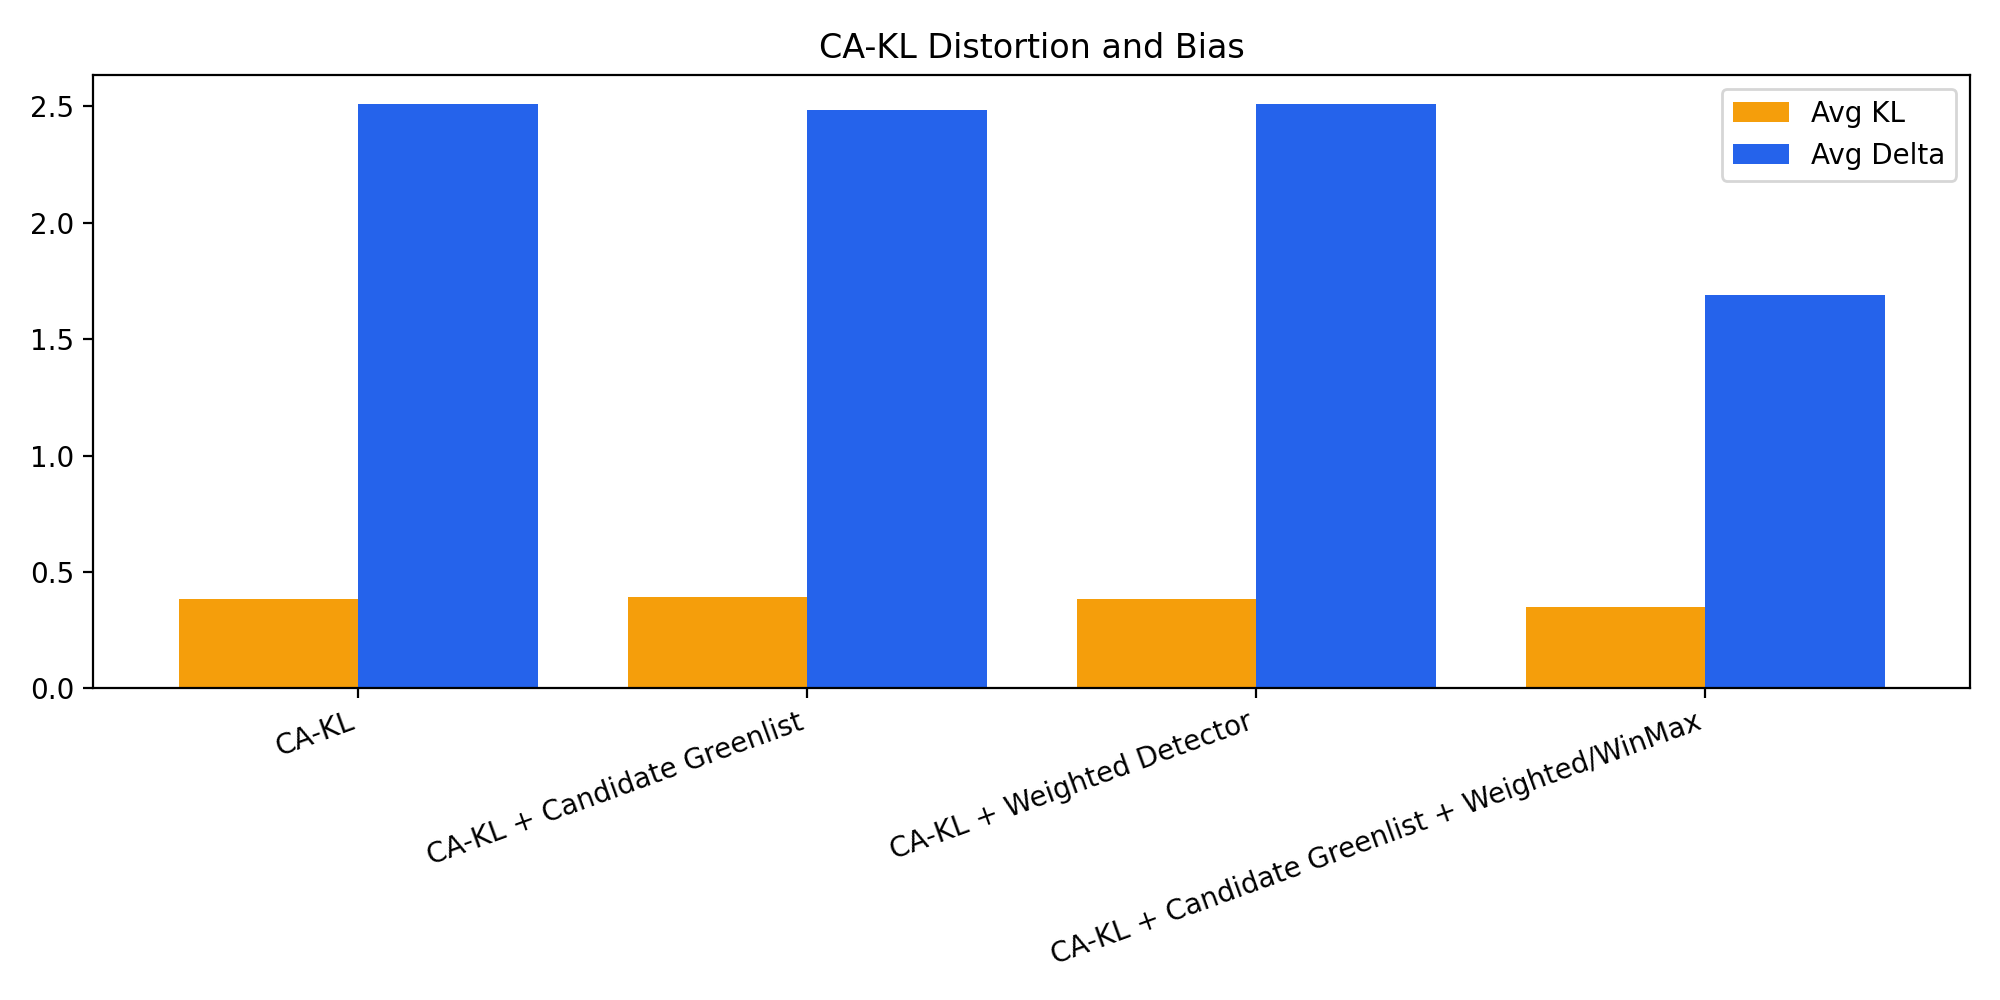
\includegraphics[width=0.86\textwidth]{cakl_kl_delta.png}
    \caption{CA-KL 方法中的平均 KL 与平均自适应 delta}
    \label{fig:kl-delta}
\end{figure}

KL 预算和 confidence gate 共同决定最终扰动强度。预算越大，可用偏置上界越高；gate 越严格，实际施加偏置的位置越少。\fullmethod{} 在 gate 0.10/0.95 下的平均 \texttt{delta} 约为 1.69，低于 \method{} 的 2.51，但在 weighted detector 下仍保持较高检测分数。这说明 KL 预算负责约束单步分布扰动，confidence gate 负责筛选适合嵌入的位置，两者共同构成完整的自适应水印强度控制机制。

为避免只以平均 \texttt{delta} 推断质量--检测折中，本文在相同 500 条 C4/realnewslike prompt、相同采样设置下扫描 $\varepsilon\in\{0.20,0.30,0.35,0.40,0.50\}$。表 \ref{tab:pareto-full} 的 KL、\texttt{delta} 和分位数均来自逐生成位置的真实记录；P25/P50/P75 为先在单条序列内计算、再在样本间平均的分位数。

\begin{table}[H]
    \centering
    \caption{500 条 prompt 上 Fixed Delta 与 CA-KL 的质量--检测比较}
    \label{tab:pareto-full}
    \scriptsize
    \setlength{\tabcolsep}{3pt}
    \begin{tabularx}{\textwidth}{p{0.24\textwidth}rrrrrr}
        \toprule
        方法 / 参数                          & PPL$\downarrow$ & KGW 检出率$\uparrow$ & 平均 z  & 平均 KL  & 平均 $\delta$ & P25/P50/P75       \\
        \midrule
        Fixed $\delta=1.0$               & 4.4996          & 25.40\%           & 2.941 & --     & 1.000       & 1.000/1.000/1.000 \\
        Fixed $\delta=1.7$               & 4.9519          & 82.00\%           & 5.535 & --     & 1.700       & 1.700/1.700/1.700 \\
        Fixed $\delta=1.864$             & 5.2054          & 89.60\%           & 6.335 & --     & 1.864       & 1.864/1.864/1.864 \\
        Fixed $\delta=2.0$               & 5.4301          & 92.80\%           & 6.820 & --     & 2.000       & 2.000/2.000/2.000 \\
        \method{} $\varepsilon=0.20$     & 4.8395          & 67.80\%           & 4.528 & 0.1666 & 1.884       & 1.387/1.630/2.319 \\
        \method{} $\varepsilon=0.30$     & 5.2778          & 84.80\%           & 5.643 & 0.2432 & 2.130       & 1.668/1.919/2.628 \\
        \method{} $\varepsilon=0.35$     & 5.4544          & 89.20\%           & 6.307 & 0.2797 & 2.235       & 1.804/2.057/2.723 \\
        \method{} $\varepsilon=0.40$     & 5.7354          & 91.60\%           & 6.837 & 0.3172 & 2.328       & 1.920/2.172/2.809 \\
        \method{} $\varepsilon=0.50$     & 5.8431          & 95.40\%           & 7.558 & 0.3836 & 2.510       & 2.155/2.424/2.943 \\
        \fullmethod{} $\varepsilon=0.50$ & 5.6073          & 88.80\%           & 6.387 & 0.3481 & 1.689       & --                \\
        \bottomrule
    \end{tabularx}
\end{table}

图 \ref{fig:pareto-kgw} 表明，随着预算增加，CA-KL 沿着“更高 PPL--更高检出率”方向连续移动；图 \ref{fig:epsilon-curves} 验证平均实际 KL 与平均 \texttt{delta} 均单调增加。更重要的是，CA-KL 没有在当前设置下严格 Pareto 支配 Fixed Delta：$\varepsilon=0.20$ 的 PPL 为 4.8395、检出率为 67.80\%，低于 PPL 相近的 Fixed $\delta=1.7$ 的 82.00\%；$\varepsilon=0.35$ 的 PPL 为 5.4544、检出率为 89.20\%，也未同时优于 Fixed $\delta=1.864$。因此，实验支持“KL 预算提供可解释的连续控制”，但不支持“其在所有质量约束下优于固定偏置”的更强断言。

\begin{figure}[H]
    \centering
    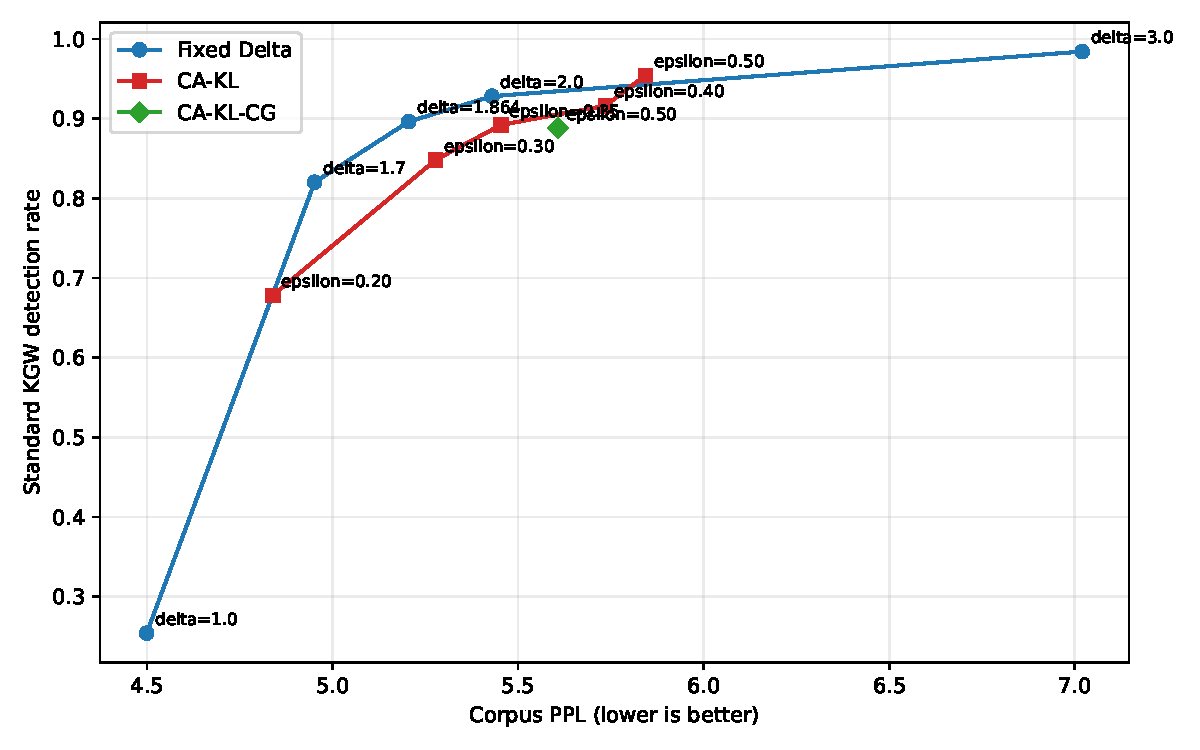
\includegraphics[width=0.82\textwidth]{pareto_ppl_kgw.pdf}
    \caption{PPL--普通 KGW 检出率 Pareto 图}
    \label{fig:pareto-kgw}
\end{figure}

\begin{figure}[H]
    \centering
    \begin{subfigure}{0.48\textwidth}
        \centering
        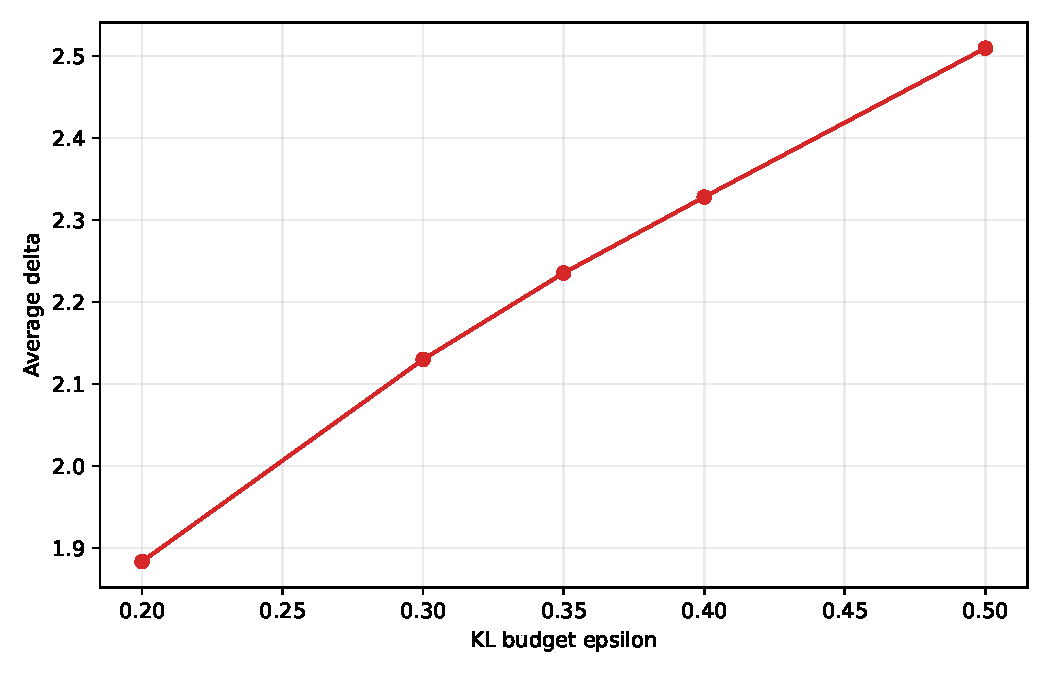
\includegraphics[width=\textwidth]{pareto_epsilon_delta.pdf}
        \caption{$\varepsilon$--平均 \texttt{delta}}
    \end{subfigure}
    \hfill
    \begin{subfigure}{0.48\textwidth}
        \centering
        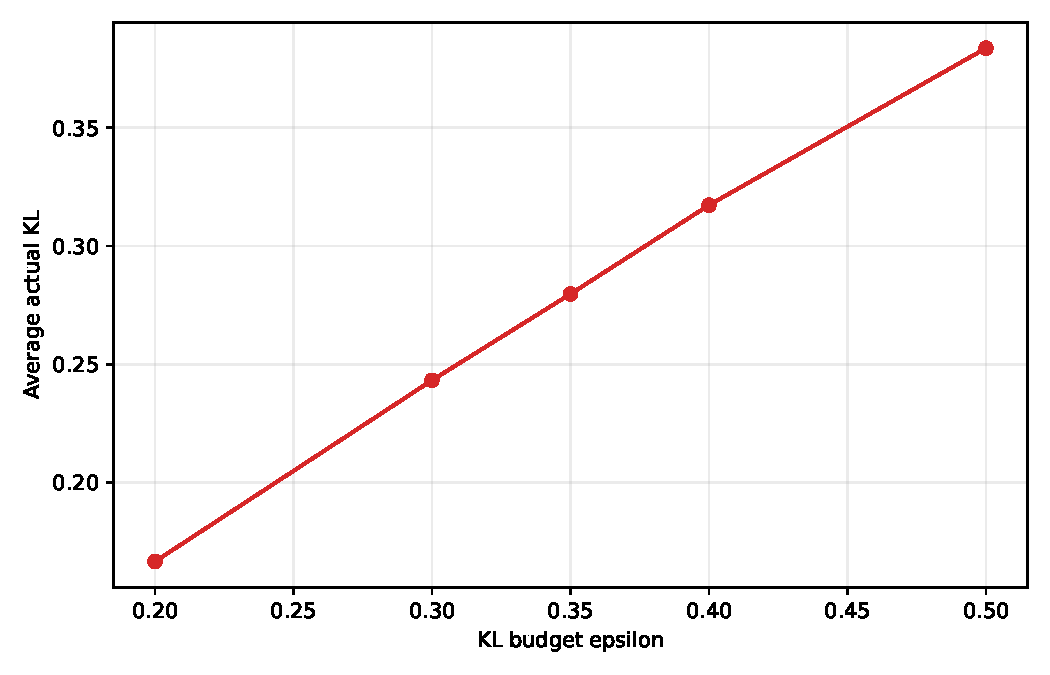
\includegraphics[width=\textwidth]{pareto_epsilon_kl.pdf}
        \caption{$\varepsilon$--平均实际 KL}
    \end{subfigure}
    \caption{KL 预算与自适应强度关系}
    \label{fig:epsilon-curves}
\end{figure}

\noindent\textbf{Copy-paste 局部混入攻击。}

本文直接复用已有生成文本，在 token 级构造固定 200 scored tokens 的攻击样本：无水印前缀、指定比例的水印片段和无水印后缀，并设置 beginning、middle、end 三个插入位置。对 Fixed Delta 2.0、\method{} 和 \fullmethod{} 各构造 500 条样本、五个比例和三个位置，共评分 22,500 条攻击文本；WinMax 使用默认窗口集合 $\{20,40,80,\mathrm{max}\}$。

表 \ref{tab:copy-paste} 合并三个插入位置。为保持攻击构造一致，表中 TPR@1\%FPR 由同构 0\% 攻击负样本得到，属于诊断值，不能替代前述五折独立校准；固定阈值检测率和分数曲线直接体现了水印信号被无水印文本稀释的程度。

\begin{table}[H]
    \centering
    \caption{Copy-paste 攻击下的 TPR@1\%FPR 诊断值（位置合并，1,500 条/比例）}
    \label{tab:copy-paste}
    \small
    \begin{tabularx}{\textwidth}{p{0.30\textwidth}rrrr}
        \toprule
        生成方法            & 水印占比 & Standard KGW & Global Weighted & WinMax  \\
        \midrule
        Fixed Delta 2.0 & 25\% & 46.27\%      & 69.80\%         & 95.13\% \\
        \method{}       & 25\% & 54.13\%      & 74.67\%         & 94.67\% \\
        \fullmethod{}   & 25\% & 43.07\%      & 61.33\%         & 88.60\% \\
        Fixed Delta 2.0 & 50\% & 95.13\%      & 97.13\%         & 99.00\% \\
        \method{}       & 50\% & 96.33\%      & 97.27\%         & 99.00\% \\
        \fullmethod{}   & 50\% & 91.93\%      & 95.47\%         & 97.60\% \\
        \bottomrule
    \end{tabularx}
\end{table}

水印比例从 100\% 降至 25\% 时，global detector 的分数与检出率明显下降，WinMax 的下降更慢。以 \fullmethod{} 为例，25\% 时 standard/global/WinMax 的平均分数为 1.892/2.628/5.551，WinMax TPR 为 88.60\%，高于 global 和 standard 的 61.33\% 与 43.07\%。在水印片段位于中间时，\fullmethod{} 的 WinMax TPR 仍为 90.20\%，说明该优势并非只来自文本起始位置。多窗口搜索的代价是需要独立校准：本攻击构造下无水印文本的 WinMax 固定阈值误报约为 0.33\%。

\begin{figure}[H]
    \centering
    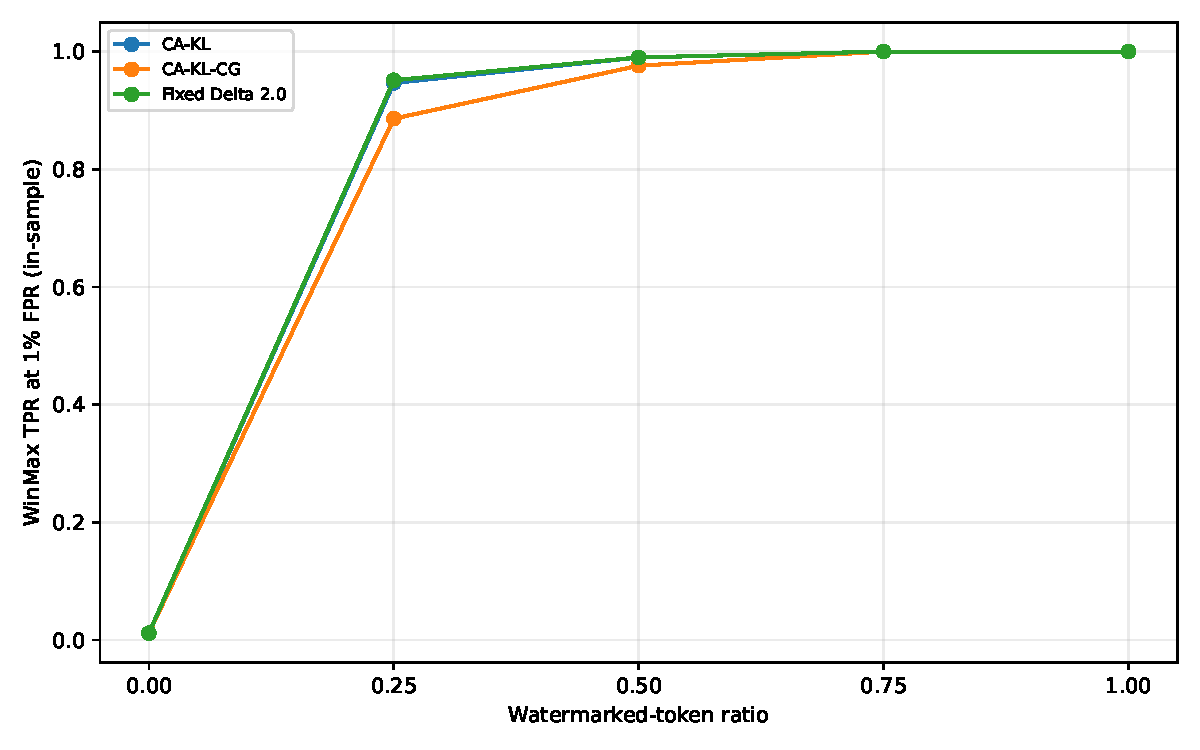
\includegraphics[width=0.82\textwidth]{copy_paste_tpr1.pdf}
    \caption{水印占比与 WinMax TPR@1\%FPR 诊断值}
    \label{fig:copy-tpr}
\end{figure}

\begin{figure}[H]
    \centering
    \begin{subfigure}{0.48\textwidth}
        \centering
        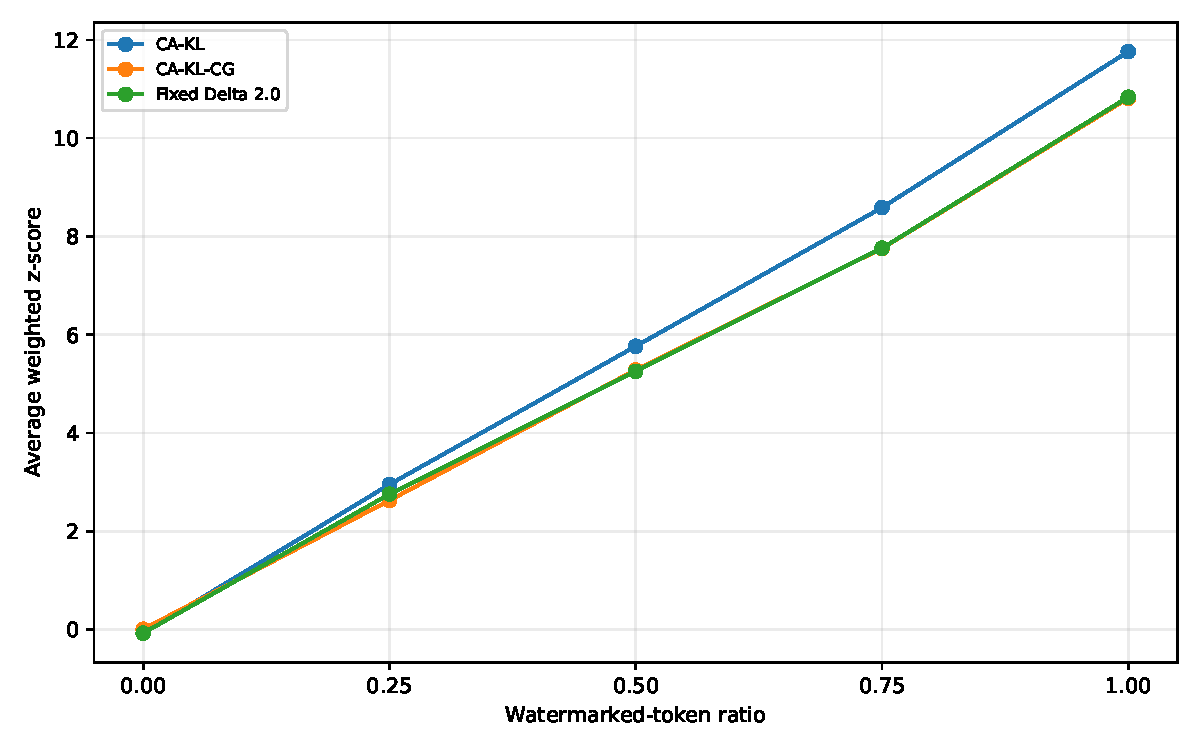
\includegraphics[width=\textwidth]{copy_paste_weighted.pdf}
        \caption{Global weighted 分数}
    \end{subfigure}
    \hfill
    \begin{subfigure}{0.48\textwidth}
        \centering
        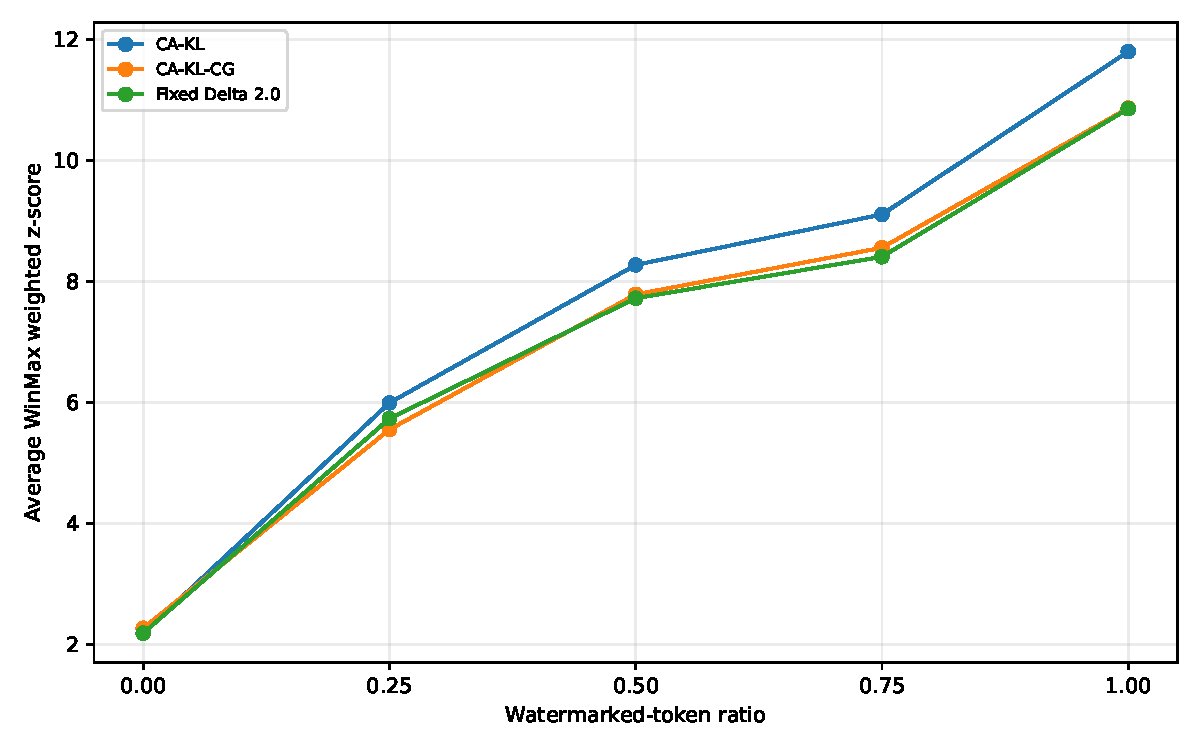
\includegraphics[width=\textwidth]{copy_paste_winmax.pdf}
        \caption{WinMax 分数}
    \end{subfigure}
    \caption{水印占比与两类模型辅助检测分数}
    \label{fig:copy-scores}
\end{figure}

\begin{figure}[H]
    \centering
    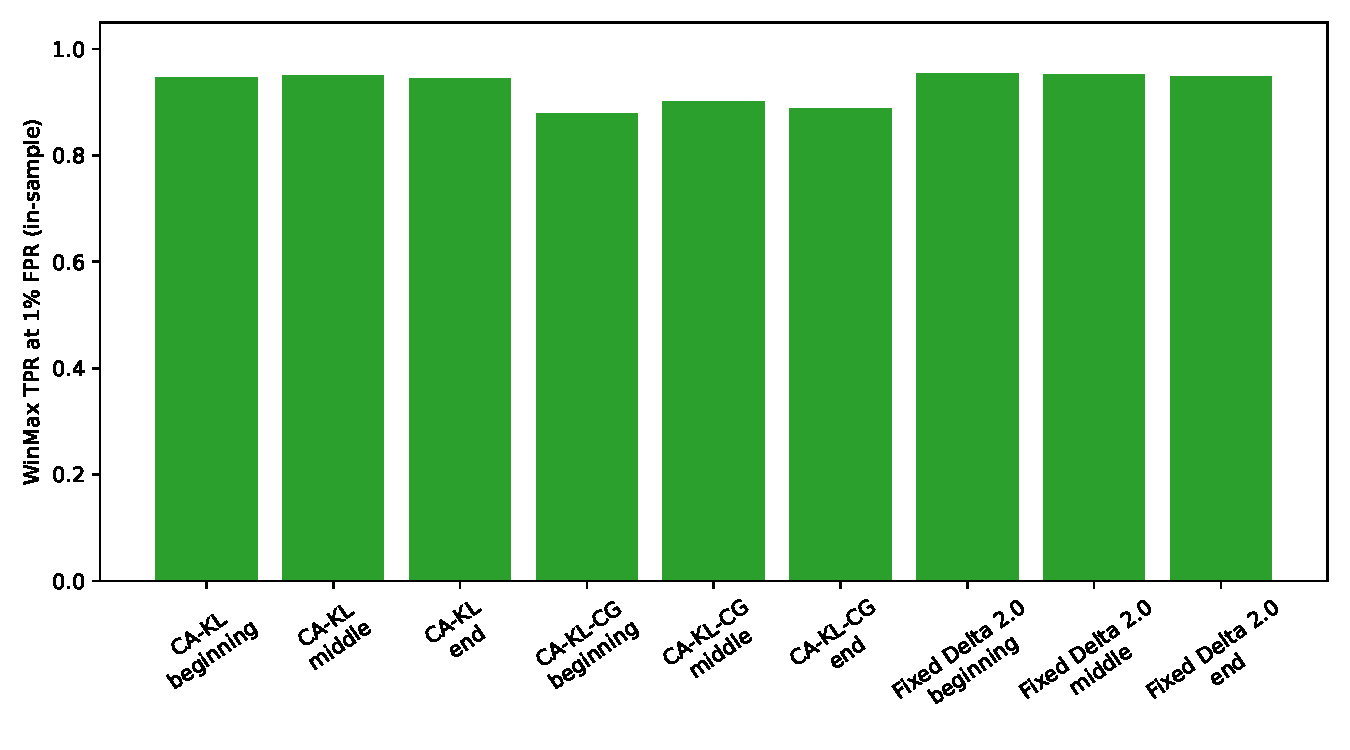
\includegraphics[width=0.86\textwidth]{copy_paste_position.pdf}
    \caption{25\% 水印占比下不同插入位置的 WinMax TPR@1\%FPR 诊断值}
    \label{fig:copy-position}
\end{figure}

\section{总结}

本报告完成了 KGW 文本水印方法的复现，并在固定 \texttt{delta} 的基础上实现了两类自适应水印机制。Adaptive Delta 通过 next-token 分布熵调整偏置强度，提供了直观的可嵌入性建模；\method{} 则进一步使用 KL 散度预算约束每一步分布扰动，使水印强度具有明确的统计解释。\fullmethod{} 在此基础上加入 candidate-aware greenlist 和 confidence gate，把水印嵌入集中到候选空间内更合适的位置。

首先，主表已经前置为 \texttt{OPT-1.3B + C4/realnewslike + 200$\pm$5 tokens + standard KGW detector} 的复现实验。两条线的平均 \texttt{tokens\_scored} 分别为 203.82 和 203.96，说明生成长度控制已经回到原论文量级；\texttt{Fixed Delta 2.0} 的 z-score 达到 10.6006、检出率达到 96.19\%，同时 continuation PPL 从 3.8492 上升到 4.9195。这一组结果更准确地回答了“我们本地是否真的复现了官方实验”这个问题，也说明此前与原论文差距较大的关键原因，确实包括模型规模、prompt 构造方式和生成长度控制不一致。

其次，改进方法已按原论文控制变量重新运行：相同的 OPT-1.3B、499 个有效 C4/realnewslike prompt、200$\pm$5 token 与 standard KGW detector，PPL 统一由 OPT-2.7B 评测。\method{} 的普通 KGW z-score 为 12.1205、检出率为 98.40\%，高于 \texttt{Fixed Delta 2.0} 的 10.6572 和 97.39\%，代价是 PPL 从 5.7426 升至 6.3104。\fullmethod{} 将嵌入位置压缩到 69.44\%，PPL 为 6.1984、检出率为 97.19\%。五折独立校准下，\method{} 的 standard z-score AUC 为 0.9954、TPR@1\%FPR 为 98.40\%，实际 FPR 为 1.40\%。这说明 KL 约束更擅长增强检测信号；confidence gate 则提供了降低平均扰动的折中，而非严格 Pareto 支配。

完整 KL 扫描给出了更审慎的结论：CA-KL 能通过 $\varepsilon$ 连续控制实际 KL、\texttt{delta}、PPL 和检测率，但在当前 OPT-2.7B/C4 设置下，尚未在所有相近 PPL 约束下严格优于 Fixed Delta。copy-paste 攻击则验证了 WinMax 的适用性：当水印片段仅占 25\% 时，WinMax 明显优于 global weighted 与 standard KGW；但多窗口搜索必须采用独立负样本阈值校准。

本文的主要贡献包括：第一，复现并系统比较固定 \texttt{delta}、Adaptive Delta、\method{} 和 \fullmethod{}；第二，提出 KL 预算下的动态水印强度控制机制，使每一步 \texttt{delta} 由分布扰动约束决定；第三，实现 candidate-aware greenlist、confidence gate 与模型辅助 weighted/WinMax detector，并以五折校准和局部混入攻击检验检测结论。

\section{实验分工}

\noindent\textbf{施煌：}负责 KGW 原论文阅读、官方仓库复现与实验设置整理，完成 C4/realnewslike prompt 构造、原论文口径的 Fixed Delta 基线核验，以及报告中方法背景、复现步骤和实验设置部分的撰写与整合。

\noindent\textbf{祖裕柏：}负责自适应生成端实现，包括基于熵的 Adaptive Delta、CA-KL 的逐位置 KL 预算二分求解、candidate-aware greenlist 和 confidence gate；编写并维护批量生成、PPL 评测和控制变量主实验脚本，完成 OPT-1.3B 主实验与 KL 预算扫描。

\noindent\textbf{黄镇邦：}负责检测与结果分析模块，实现 weighted detector、WinMax detector、五折独立阈值校准和 bootstrap 统计；完成 copy-paste 局部混入攻击、实验图表与结果汇总，并参与实验结果、局限性和结论部分的撰写。


\clearpage
\bibliographystyle{ieeetr}
\bibliography{reference}

\appendix
\section{核心代码片段}

下面列出 \method{} 中 KL 约束求解的核心逻辑。

\begin{lstlisting}[language=Python]
def _kl_for_delta(self, delta: float, p_green_mass: float) -> float:
    if delta <= 0.0 or p_green_mass <= 0.0:
        return 0.0
    normalizer = 1.0 + (exp(delta) - 1.0) * p_green_mass
    q_green_mass = exp(delta) * p_green_mass / normalizer
    return delta * q_green_mass - log(normalizer)

def _solve_delta(self, p_green_mass: float) -> tuple[float, float]:
    if self.kl_epsilon <= 0.0 or self.delta_max <= 0.0:
        return 0.0, 0.0
    if self._kl_for_delta(self.delta_max, p_green_mass) <= self.kl_epsilon:
        return self.delta_max, self._kl_for_delta(self.delta_max, p_green_mass)
    lo, hi = 0.0, self.delta_max
    for _ in range(self.binary_search_steps):
        mid = (lo + hi) / 2.0
        if self._kl_for_delta(mid, p_green_mass) <= self.kl_epsilon:
            lo = mid
        else:
            hi = mid
    return lo, self._kl_for_delta(lo, p_green_mass)
\end{lstlisting}

\end{document}
